\documentclass[aspectratio=169,10pt]{beamer}
\usepackage[utf8]{inputenc}
\usepackage[T1]{fontenc}
\usepackage[spanish,es-nodecimaldot]{babel}
\usepackage{graphicx,booktabs}
\definecolor{Direccion}{HTML}{185879}
\setbeamercolor{structure}{fg=Direccion}
\setbeamercolor{frametitle}{fg=white,bg=Direccion}
\setbeamertemplate{navigation symbols}{}
\setbeamertemplate{footline}{\hfill\scriptsize Alto Atoyac | Presentación a dirección\hspace{1em}\insertframenumber/\inserttotalframenumber\hspace{1em}\vspace{2mm}}
\setbeamersize{text margin left=7mm,text margin right=7mm}
\title{Marco territorial de establecimientos\\potencialmente relevantes}
\subtitle{Hallazgos, filtros y modalidades\\de distribución y concentración territorial}
\author{Proyecto Alto Atoyac | Presentación a dirección}
\date{17 de septiembre de 2026}
\begin{document}
\begin{frame}\titlepage\end{frame}
\begin{frame}{Qué entrega este estudio a dirección}
\small
\begin{itemize}
\item Un marco territorial reproducible para localizar establecimientos potencialmente relevantes y orientar la fase enfocada en lavanderías industriales.
\item Cinco modalidades permiten observar cuánto depende el resultado del filtro de lavanderías y de la integración de información MH.
\item El marco permite comparar cobertura, distribución y concentración de establecimientos según los criterios de selección.
\item Los conteos describen candidatos y evidencia disponible; no estiman consumo, descarga ni contaminación.
\end{itemize}
\end{frame}
\begin{frame}{Hallazgos que cambian la decisión}
\small
\begin{itemize}
\item El escenario amplio DENUE contiene 1,679 candidatos; el estricto DENUE, 469. La regla de lavanderías cambia 1,210 registros.
\item MH incorpora 38 registros al amplio y 41 al estricto; su aporte es localizado y recupera casos que las reglas no retienen.
\item El escenario estricto con MH reúne 510 candidatos; 419 quedan en REVISAR y 91 en SI bajo las etiquetas actuales.
\item Recomendación: usar estricto + MH para priorizar, acompañado del amplio para mostrar sensibilidad y conservando la procedencia de cada registro.
\end{itemize}
\end{frame}
\begin{frame}{Alcance: territorio, fecha y denominador}
\small
\begin{itemize}
\item Fuente estatal del flujo actual: INEGI\_DENUE\_11092026.csv; 15,956 registros descargados. El nombre del archivo indica la fecha de descarga, no demuestra la fecha de observación de cada registro.
\item La descarga es sectorial (carpeta 313-314-315-81); no representa todas las actividades económicas de Puebla.
\item Se seleccionan 26 municipios por nombre normalizado; 24 tienen candidatos en las tablas de cobertura.
\item Después se intersectan puntos con el polígono de cuenca. Cada cifra comparativa principal usa este mismo recorte dentro de la cuenca.
\item El alcance es el territorio trabajado de Puebla. No se debe presentar como inventario de toda la cuenca en ambos estados.
\end{itemize}
\end{frame}
\begin{frame}{Territorio y red hidrográfica}
\centering
\includegraphics[width=.97\textwidth,height=.72\textheight,keepaspectratio]{../outputs/cuenca_alto_atoyac_puebla_estricto_mh/maps/png/01_cuenca_informacion_hidrica.png}
\par\scriptsize Fuente: capas de cuenca, municipios y red hidrográfica incluidas en el proyecto; mapa del flujo 08.
\end{frame}
\begin{frame}{Arquitectura completa del procedimiento}
\small
\begin{itemize}
\item 1. Leer y normalizar DENUE; validar columnas e identificadores; construir puntos.
\item 2. Ejecutar por separado filtro SCIAN y filtro textual; unir identificadores sin duplicar establecimientos.
\item 3. Interpretar señales y asignar decisión sectorial y evidencia hídrica, como dimensiones distintas.
\item 4. Seleccionar municipios; aplicar el corte hídrico de la modalidad; guardar el resultado previo a MH.
\item 5. Integrar MH cuando corresponde; recortar puntos por cuenca; calcular distancia y agregaciones.
\item 6. Exportar tablas CSV, capas GPKG, mapas PNG/HTML e inventarios. Esta presentación reutiliza esas salidas y añade comparaciones.
\end{itemize}
\end{frame}
\begin{frame}{Proceso 1: lectura, normalización y controles}
\small
\begin{itemize}
\item El flujo estatal lee el CSV como texto con codificación cp1252 y sustituye nulos por cadenas vacías.
\item Normaliza acentos en encabezados y renombra ID, nombre, razón social, SCIAN y localidad a los campos internos.
\item Exige ID, nombre, razón social, código y descripción SCIAN, municipio, localidad, latitud, longitud y estrato de personal.
\item Rechaza identificadores duplicados; elimina espacios exteriores de los campos clave.
\item Convierte longitud y latitud a números, construye puntos en EPSG:4326 y comprueba geometrías nulas.
\item Límite del control actual: no incorpora una comprobación explícita de rangos geográficos, vigencia de operación o coordenadas plausibles para Puebla.
\end{itemize}
\end{frame}
\begin{frame}{Proceso 2A: filtro estructurado SCIAN}
\small
\begin{itemize}
\item Normaliza el código como texto, elimina el sufijo .0 y espacios.
\item Retiene códigos que comienzan con 313, 314, 315 o 812210. El operador es coincidencia de prefijo.
\item Los prefijos 313/314/315 definen contexto sectorial textil en las reglas; no prueban proceso húmedo.
\item El código exacto 313310 genera la señal scian\_acabado\_humedo; el exacto 812210 genera scian\_lavanderia.
\item 812210 no distingue por sí solo lavandería comercial de lavandería industrial.
\item El filtro solo puede recuperar establecimientos presentes en la descarga: ampliar palabras no recupera actividades ausentes del archivo fuente.
\end{itemize}
\end{frame}
\begin{frame}{Proceso 2B: texto que efectivamente se analiza}
\small
\begin{itemize}
\item Se concatena nombre del establecimiento + razón social. Se pasa a minúsculas, se eliminan acentos y se normalizan espacios.
\item La descripción SCIAN se exige como columna, pero está comentada en la construcción de texto\_filtro; no se analiza en el filtro textual actual.
\item El catálogo giro\_textil.csv vincula cada palabra o frase con una señal; una frase puede generar más de una señal.
\item Se buscan palabras o frases completas mediante límites alfanuméricos; las frases largas se ordenan primero y los espacios se flexibilizan.
\item Limitaciones: nombres comerciales poco descriptivos, abreviaturas y variantes no incluidas pueden perder señales; palabras generales pueden crear coincidencias ambiguas.
\end{itemize}
\end{frame}
\begin{frame}{Diccionario: contexto textil y productivo}
\small
\begin{itemize}
\item textil: 48 entradas. Ejemplos: acabado textil, bordado, bordados, confeccion, confecciones
\item mezclilla: 20 entradas. Ejemplos: acid wash, denim, desebrado, deshebrado, fosil
\item produccion: 37 entradas. Ejemplos: bordado, bordados, confeccion, confeccion en serie, confecciones
\item maquila: 11 entradas. Ejemplos: confeccion en serie, ensamble de prendas, maquila, maquila de mezclilla, maquila de prendas
\item El catálogo completo se incluye al final, para que ninguna entrada quede omitida.
\end{itemize}
\end{frame}
\begin{frame}{Diccionario: procesos y exclusiones}
\small
\begin{itemize}
\item humedo\_explicito: 49 entradas. Ejemplos: acabado, acabado de prendas, acabado quimico, acabado textil, acid wash
\item lavado\_generico: 6 entradas. Ejemplos: clean clothes, laundry, lavado, lavanderia, tratamiento
\item proceso\_seco\_explicito: 10 entradas. Ejemplos: costura, confeccion, confecciones, corte, corte y confeccion
\item no\_textil\_explicito: 22 entradas. Ejemplos: captacion, tratamiento y suministro de agua, agua potable y alcantarillado, purificacion y embotellado de agua, lavado de botellas, lavado y lubricado de automoviles y camiones
\item El catálogo completo se incluye al final, para que ninguna entrada quede omitida.
\end{itemize}
\end{frame}
\begin{frame}{Proceso 2C: retención textual y exclusiones}
\small
\begin{itemize}
\item Se crean siete señales positivas: textil, mezclilla, húmedo explícito, lavado genérico, producción, maquila y proceso seco explícito.
\item El subconjunto textual retiene filas con al menos una señal positiva; una señal de proceso seco también basta para ser candidato textual.
\item Se calcula no\_textil\_explicito con el mismo texto. Una coincidencia negativa excluye del subconjunto textual aunque haya señales positivas.
\item La exclusión textual no es un veto global: una fila puede permanecer por SCIAN al efectuar la unión.
\item Las señales positivas se incorporan desde el subconjunto textual retenido. Si una fila fue excluida allí y entra por SCIAN, esas señales quedan en False.
\item Por tanto, el resultado debe explicarse como ejecución de reglas, no como auditoría de actividad real.
\end{itemize}
\end{frame}
\begin{frame}{Proceso 3: unión e identificadores}
\small
\begin{itemize}
\item Se calculan los conjuntos de ID del filtro SCIAN y del filtro textual de forma independiente.
\item Candidatos = ID SCIAN unión ID texto. Se recupera una sola fila original por ID.
\item Se guardan coincide\_filtro\_scian y coincide\_filtro\_texto para explicar por qué entró cada registro.
\item Las señales textuales se añaden con unión uno a uno; señales ausentes se convierten a False.
\item El flujo estatal actual produce 15,956 candidatos auditables: coincide con la descarga. Esto no significa que todos tengan relevancia hídrica.
\end{itemize}
\end{frame}
\begin{frame}{Proceso 4A: condiciones intermedias exactas}
\small
\begin{itemize}
\item Contexto textil = SCIAN textil o señal textil o señal mezclilla.
\item Contexto productivo = señal producción o señal maquila.
\item Evidencia húmeda = SCIAN exacto 313310 o (húmedo explícito y contexto textil).
\item Señal adicional de lavandería = textil o mezclilla o húmedo explícito o producción o maquila. Lavado genérico solo no basta en modo estricto.
\item Mezclilla relevante = mezclilla y (lavado genérico o húmedo explícito o contexto productivo).
\item Estas condiciones combinan clasificación administrativa y vocabulario; no miden intensidad del proceso.
\end{itemize}
\end{frame}
\begin{frame}{Proceso 4B: decisión sectorial}
\small
\begin{itemize}
\item Cada candidato empieza con sector\_textil = REVISAR.
\item Se asigna INCLUIR si tiene SCIAN textil; o contexto productivo y (textil o mezclilla); o evidencia húmeda.
\item La decisión sectorial y la evidencia hídrica son columnas distintas: INCLUIR no equivale a SI hídrico.
\item Una lavandería puede tener sector REVISAR y evidencia hídrica REVISAR o SI.
\item El universo hídrico estatal se selecciona por evidencia\_hidrica; no exige sector\_textil = INCLUIR como segunda condición.
\end{itemize}
\end{frame}
\begin{frame}{Proceso 4C: regla amplia y regla estricta}
\small
\begin{itemize}
\item Amplia: toda lavandería SCIAN 812210 es admisible como lavado por revisar, aun sin señal adicional.
\item Estricta: SCIAN 812210 es admisible por esa vía solo si tiene alguna señal adicional.
\item En ambas: lavado genérico y contexto textil también genera lavado por revisar. El modo estricto modifica una vía de admisión, no todos los criterios.
\item Las demás condiciones de evidencia húmeda y mezclilla relevante se mantienen.
\item Ventaja del amplio: mayor cobertura de nombres poco informativos. Ventaja del estricto: reduce ambigüedad.
\item Costo del amplio: mezcla perfiles comerciales e industriales. Costo del estricto: puede perder industriales reales sin señales en el nombre.
\end{itemize}
\end{frame}
\begin{frame}{Proceso 4D: clasificación hídrica y precedencia}
\small
\begin{itemize}
\item Cada candidato empieza como SIN\_EVIDENCIA.
\item Pasa a REVISAR si cumple lavado por revisar o mezclilla relevante.
\item Pasa a SI si cumple evidencia húmeda. Esta asignación se ejecuta después y tiene prioridad sobre REVISAR.
\item La señal proceso\_seco\_explicito no veta la evidencia húmeda ni se usa como regla final de exclusión hídrica.
\item SIN\_EVIDENCIA significa ausencia de señales bajo estas reglas, no ausencia demostrada de uso de agua.
\item SI automático significa evidencia administrativa o textual según el criterio; no confirma descarga ni carácter industrial.
\end{itemize}
\end{frame}
\begin{frame}{Ejemplos de aplicación de las reglas}\centering\scriptsize
\begin{tabular}{lll}\toprule
Caso hipotético & Amplio & Estricto\\\midrule
812210; nombre solo Lavandería Luna & REVISAR & SIN\_EVIDENCIA\\
812210; Lavandería Industrial Luna & REVISAR & REVISAR\\
812210; Lavado de mezclilla Luna & SI & SI\\
315; taller de costura sin otra señal & SIN\_EVIDENCIA & SIN\_EVIDENCIA\\
315; maquila de mezclilla & REVISAR & REVISAR\\
313310; nombre no descriptivo & SI & SI\\
\bottomrule\end{tabular}
\par\medskip Ejemplos explicativos, no establecimientos observados. Industrial genera producción/húmedo, pero SI requiere contexto textil o 313310.\end{frame}
\begin{frame}{Proceso 5: municipios y modalidades}
\small
\begin{itemize}
\item Se normalizan nombres de municipio eliminando acentos, ajustando mayúsculas y espacios; se retienen los 26 nombres solicitados.
\item Resultado común: 4,365 candidatos sectoriales en los municipios seleccionados.
\item Amplio y estricto retienen SI y REVISAR y guardan primero universo\_hidrico\_26\_municipios\_solo\_filtro.csv.
\item Con --sin-mh se mantiene solo DENUE y se registran las fuentes REGLAS\_DENUE y FILTRO\_DENUE.
\item Con --todos-scian se conservan todos los candidatos seleccionados, incluidos SIN\_EVIDENCIA, y se omite MH.
\item La modalidad sectorial conserva la unión SCIAN/texto ya calculada; el nombre todos-scian no implica un nuevo censo completo.
\end{itemize}
\end{frame}
\begin{frame}{Comparación con denominadores explícitos}\centering\scriptsize
\begin{tabular}{lllll}\toprule
Modalidad & 26 municipios & Dentro de cuenca & SI & REVISAR\\\midrule
Sectorial & 4365 & 4010 & 41 & 1638\\
Amplio DENUE & 1718 & 1679 & 41 & 1638\\
Amplio + MH & 1756 & 1717 & 91 & 1626\\
Estricto DENUE & 476 & 469 & 41 & 428\\
Estricto + MH & 517 & 510 & 91 & 419\\
\bottomrule\end{tabular}
\par\medskip Sectorial incluye además 2,331 SIN\_EVIDENCIA dentro de cuenca. Son escenarios de reglas, no intervalos estadísticos de población.\end{frame}
\begin{frame}{Sensibilidad del tamaño del universo}
\centering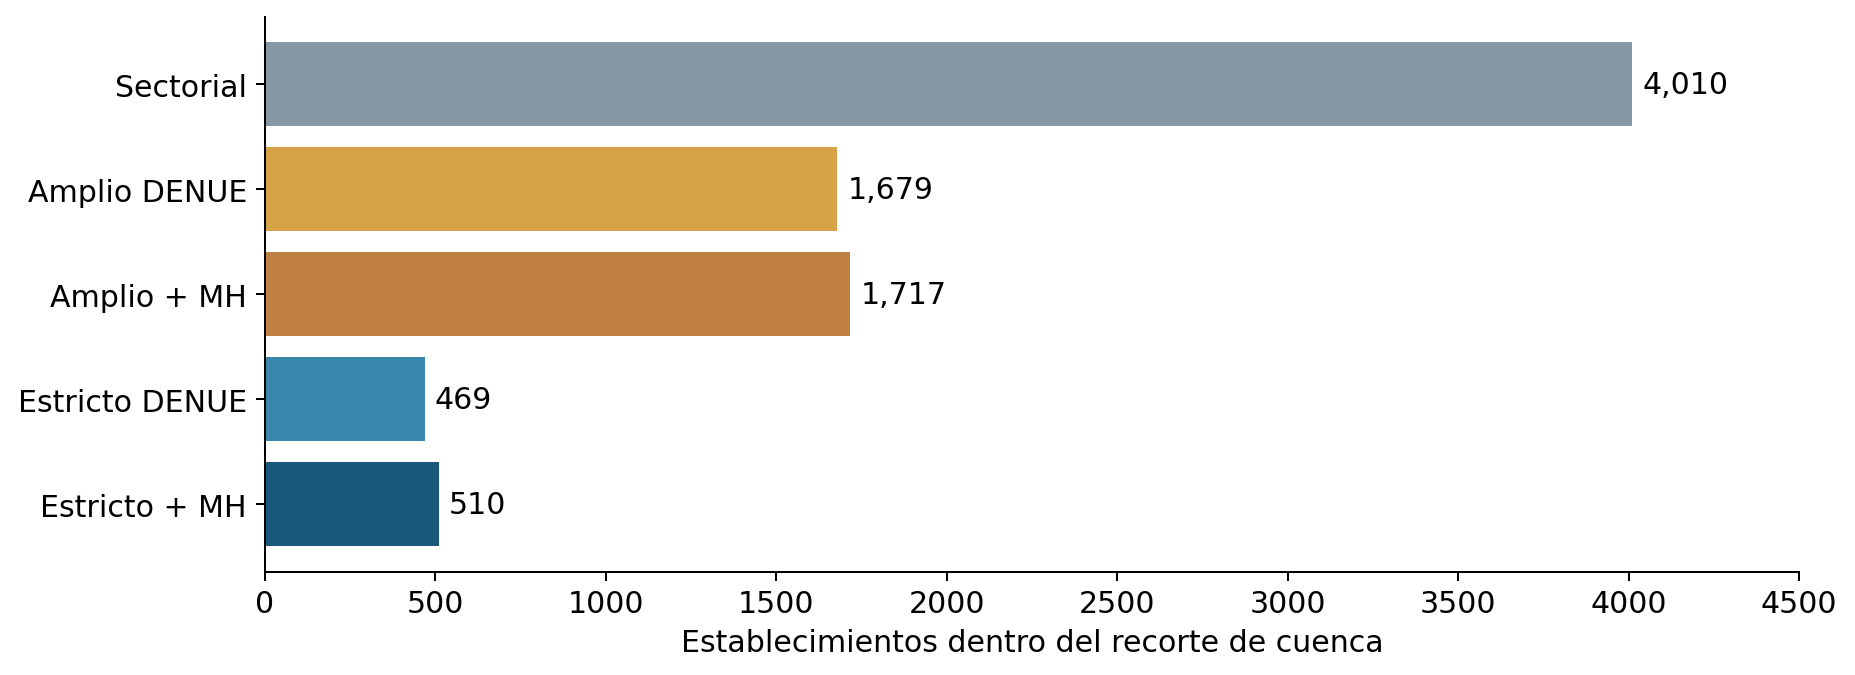
\includegraphics[width=.97\textwidth,height=.72\textheight,keepaspectratio]{direccion_imagenes/modalidades.png}
\par\scriptsize Comparación del mismo recorte espacial. La mayor diferencia corresponde a la regla de lavanderías.
\end{frame}
\begin{frame}{Cómo comparar distribución y concentración}
\small
\begin{itemize}
\item Distribución muestra cada establecimiento en su ubicación; concentración municipal suma puntos dentro de polígonos municipales recortados por cuenca.
\item Los cinco mapas de conteo usan la misma extensión, colores y escala de 0 a 1762 registros. No se ajusta la escala por modalidad.
\item El segundo panel compara participación: porcentaje del total de cada modalidad que cae en cada municipio. Permite comparar estructura territorial pese a los distintos tamaños.
\item La matriz resume conteos reales; usa log(1 + conteo) solo en el color para hacer visibles municipios pequeños.
\item La asignación espacial usa within y puede dejar puntos de límite sin asignar. Estos conteos pueden diferir del municipio declarado por DENUE.
\end{itemize}
\end{frame}
\begin{frame}{Cinco modalidades: concentración municipal absoluta}
\centering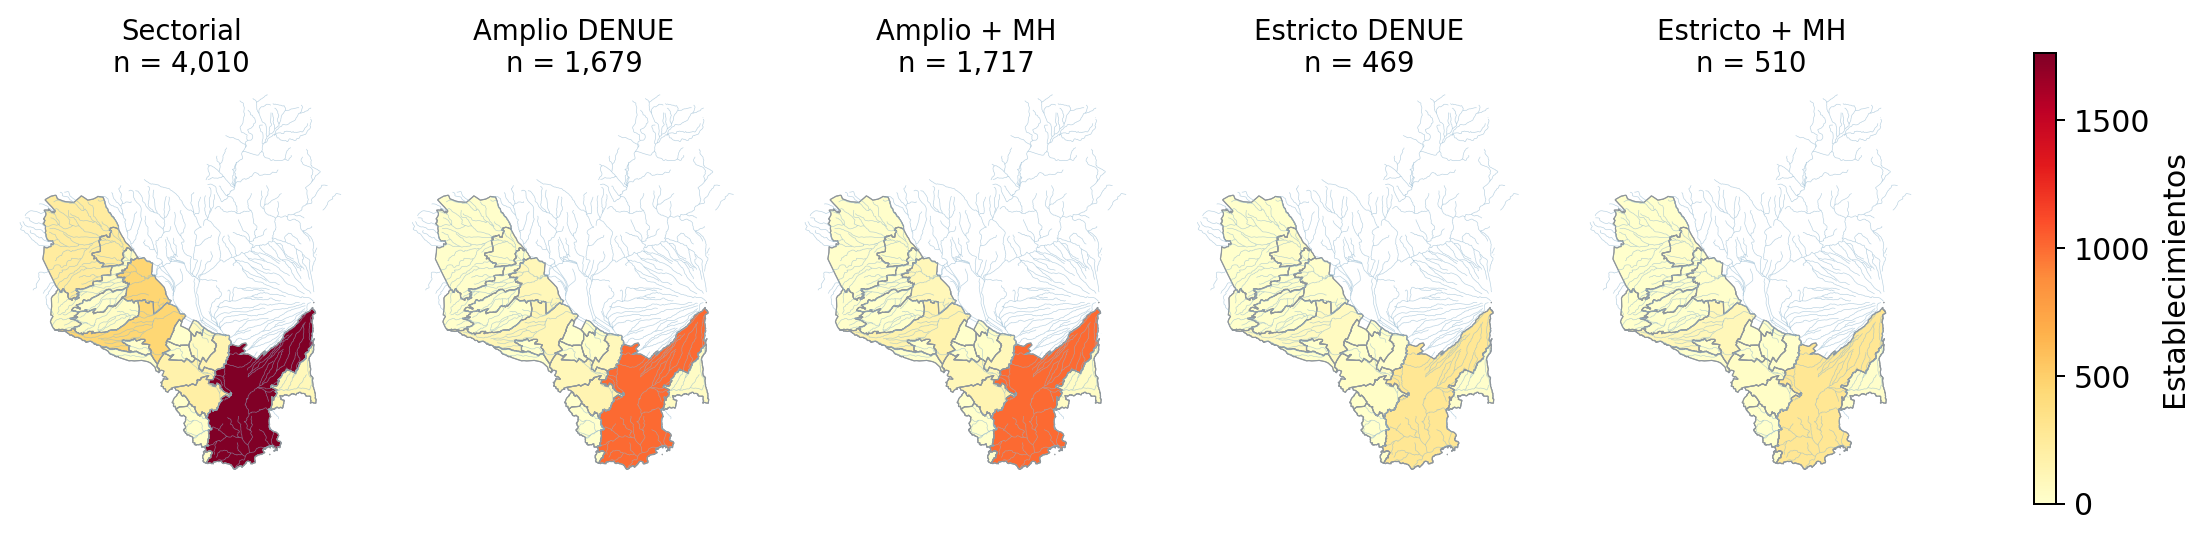
\includegraphics[width=.97\textwidth,height=.72\textheight,keepaspectratio]{direccion_imagenes/panel_conteos.png}
\par\scriptsize Escala común de conteos. Los colores comparan cantidades de establecimientos; no representan intensidad hídrica.
\end{frame}
\begin{frame}{Cinco modalidades: participación territorial}
\centering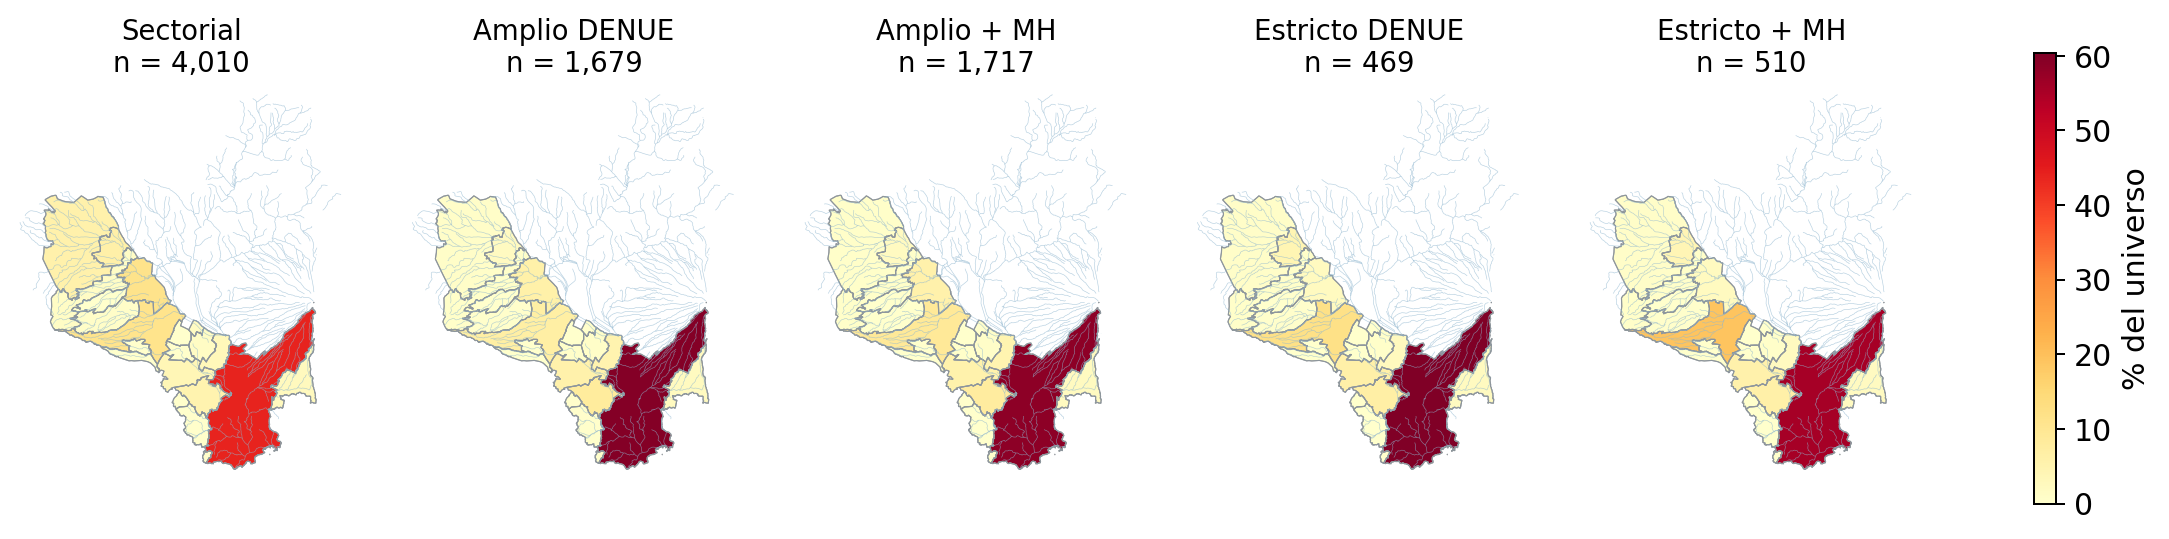
\includegraphics[width=.97\textwidth,height=.72\textheight,keepaspectratio]{direccion_imagenes/panel_participacion.png}
\par\scriptsize Escala común de porcentajes; denominador = total de registros dentro de cuenca de cada modalidad. No es densidad por km².
\end{frame}
\begin{frame}{Heatmap comparativo por municipio y modalidad}
\centering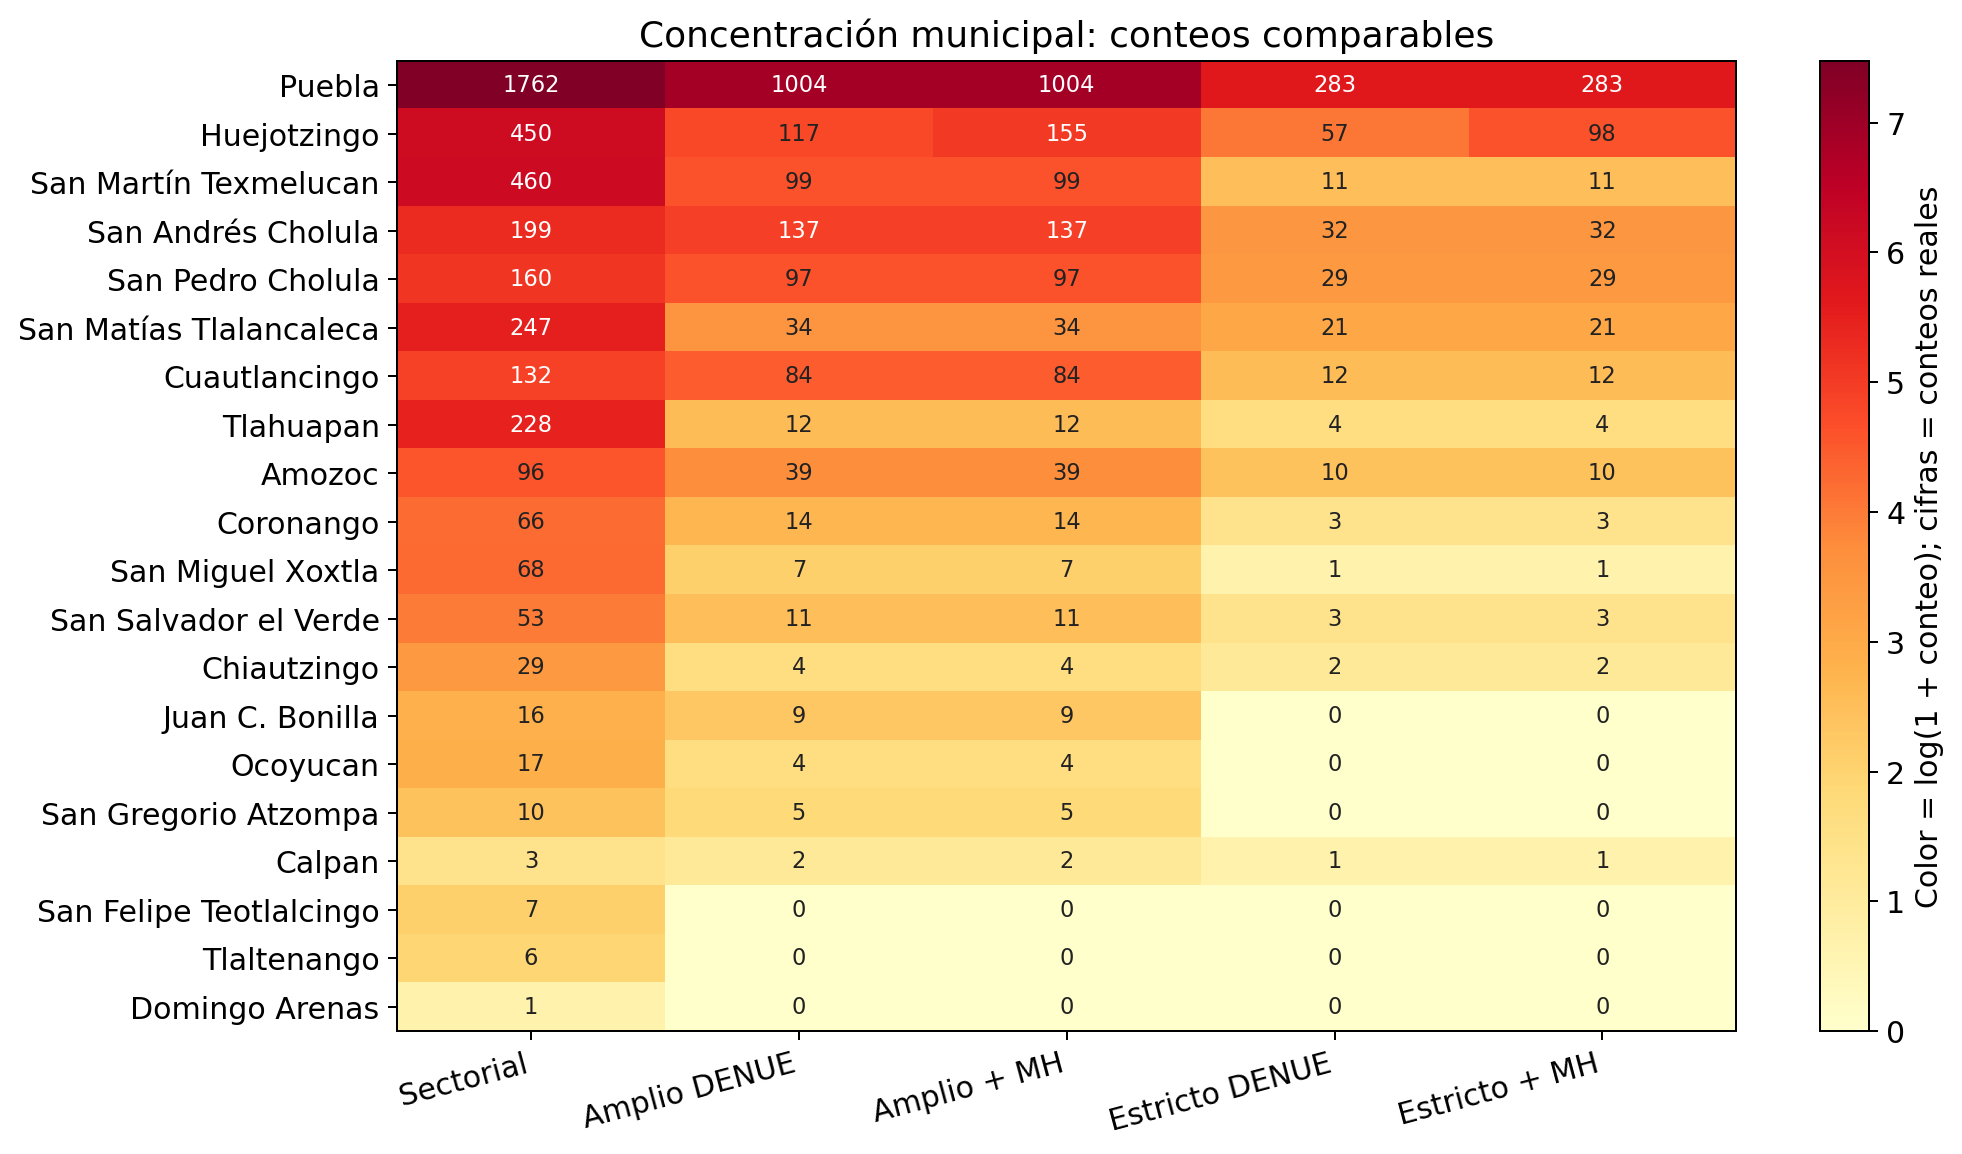
\includegraphics[width=.97\textwidth,height=.72\textheight,keepaspectratio]{direccion_imagenes/matriz_municipal.png}
\par\scriptsize Cifras = conteos espaciales. Color logarítmico para visibilidad; el orden de filas usa la suma de las cinco columnas, sin tratarla como universo único.
\end{frame}
\begin{frame}{Distribución y concentración: Sectorial}
\centering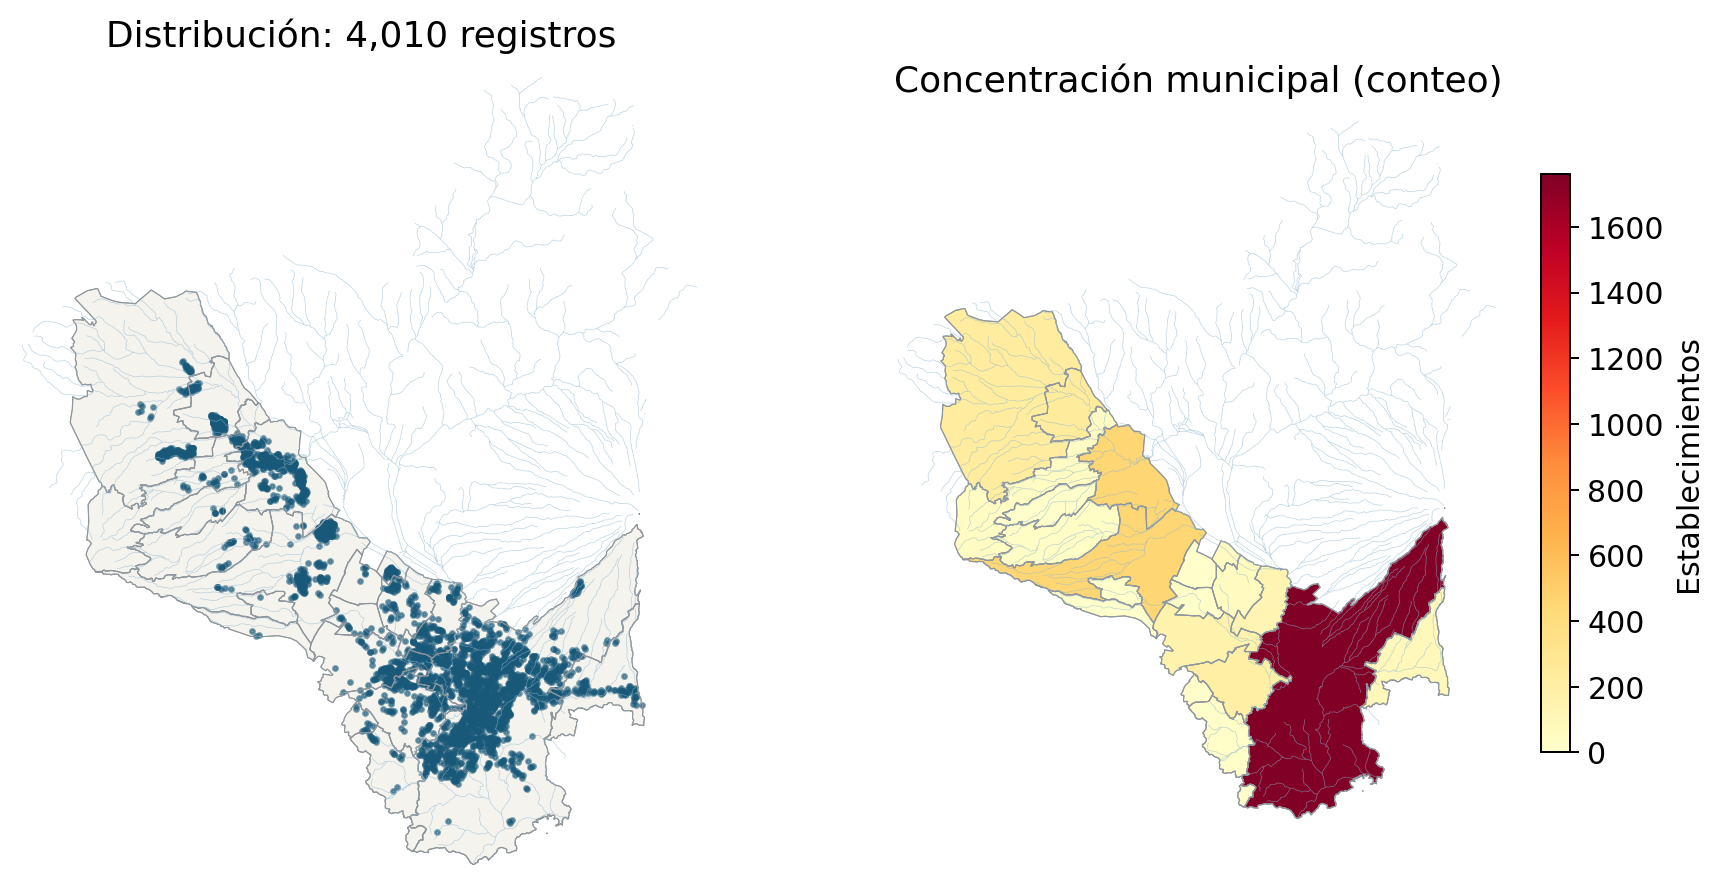
\includegraphics[width=.97\textwidth,height=.72\textheight,keepaspectratio]{direccion_imagenes/comparacion_modo_0.png}
\par\scriptsize Puntos a la izquierda; conteo por polígono a la derecha. Escala absoluta idéntica en las cinco modalidades.
\end{frame}
\begin{frame}{Distribución y concentración: Amplio DENUE}
\centering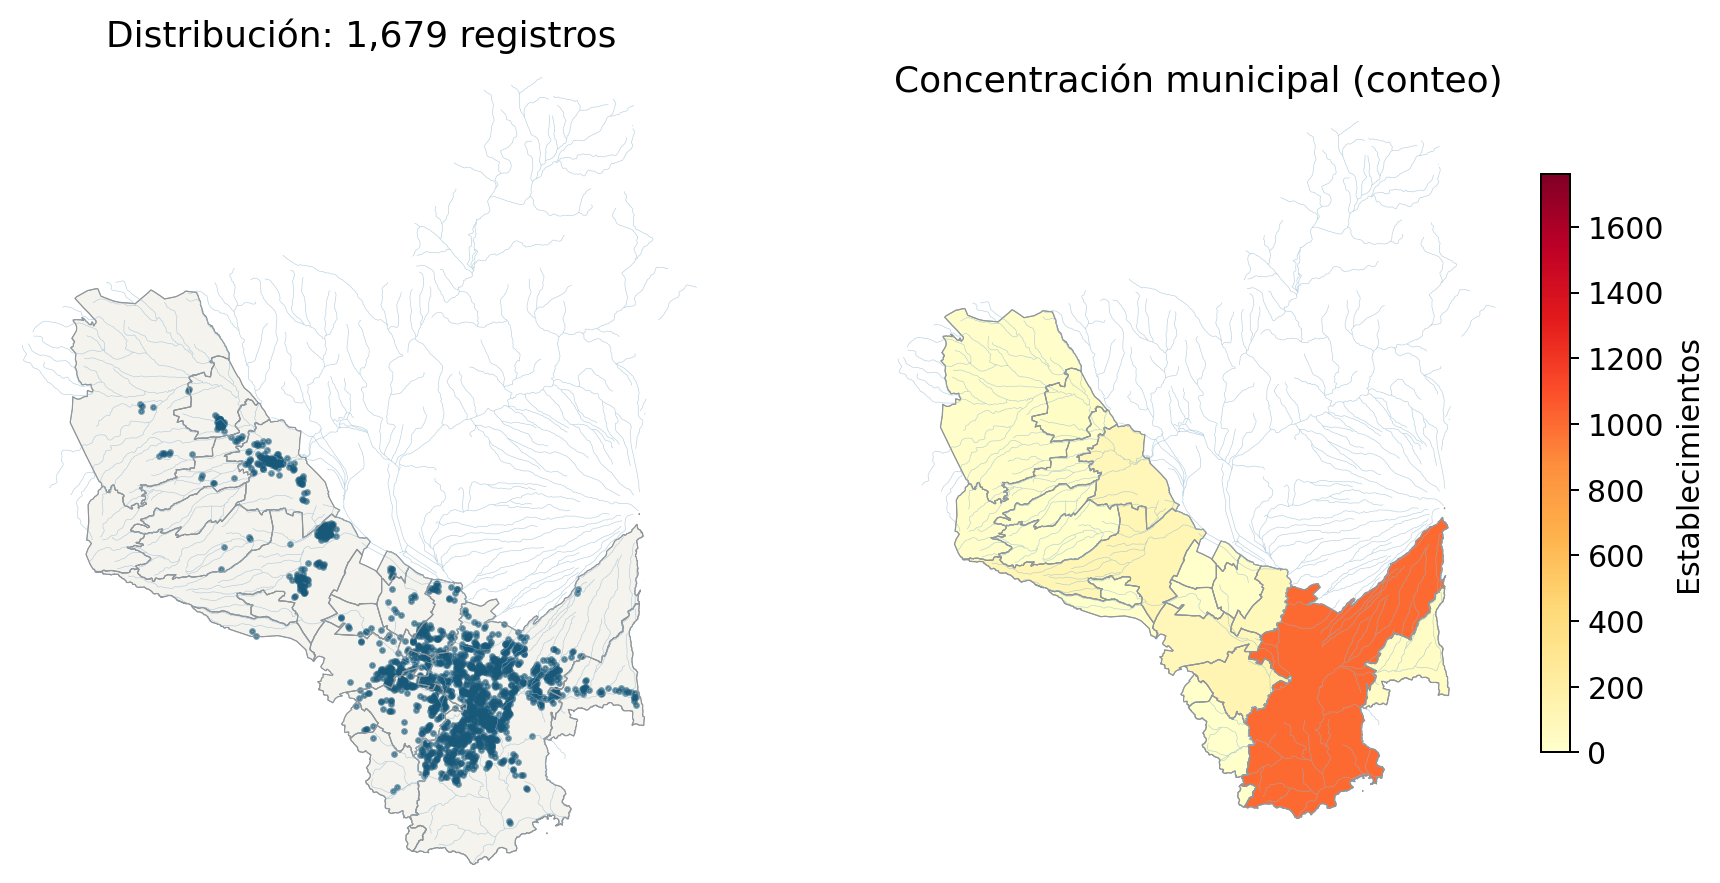
\includegraphics[width=.97\textwidth,height=.72\textheight,keepaspectratio]{direccion_imagenes/comparacion_modo_1.png}
\par\scriptsize Puntos a la izquierda; conteo por polígono a la derecha. Escala absoluta idéntica en las cinco modalidades.
\end{frame}
\begin{frame}{Distribución y concentración: Amplio + MH}
\centering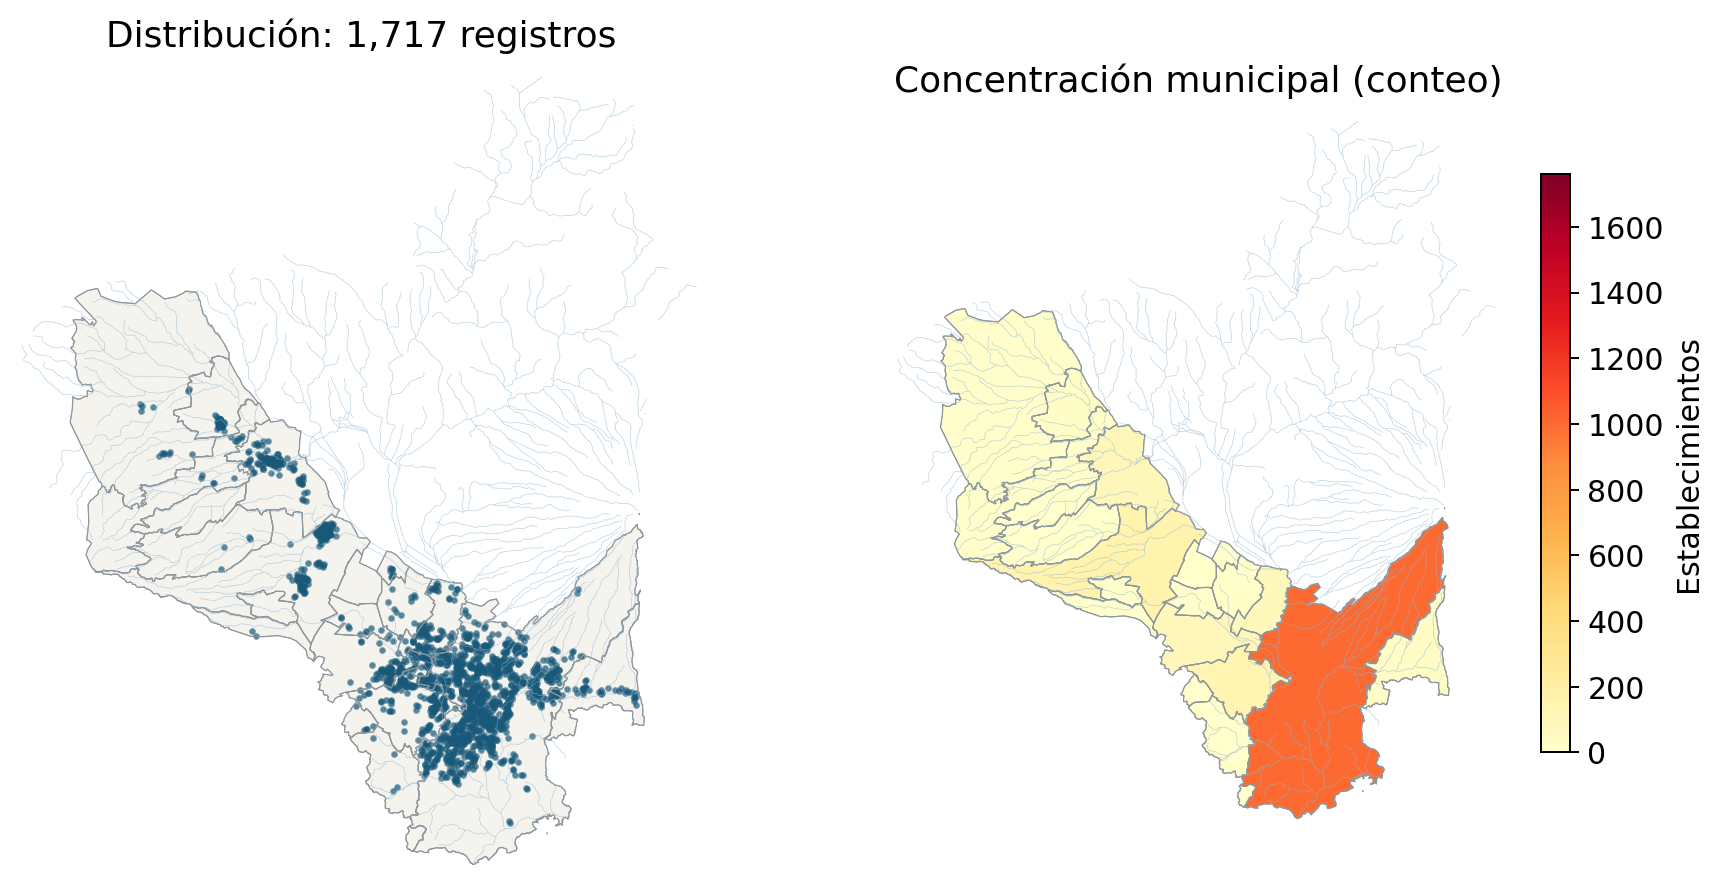
\includegraphics[width=.97\textwidth,height=.72\textheight,keepaspectratio]{direccion_imagenes/comparacion_modo_2.png}
\par\scriptsize Puntos a la izquierda; conteo por polígono a la derecha. Escala absoluta idéntica en las cinco modalidades.
\end{frame}
\begin{frame}{Distribución y concentración: Estricto DENUE}
\centering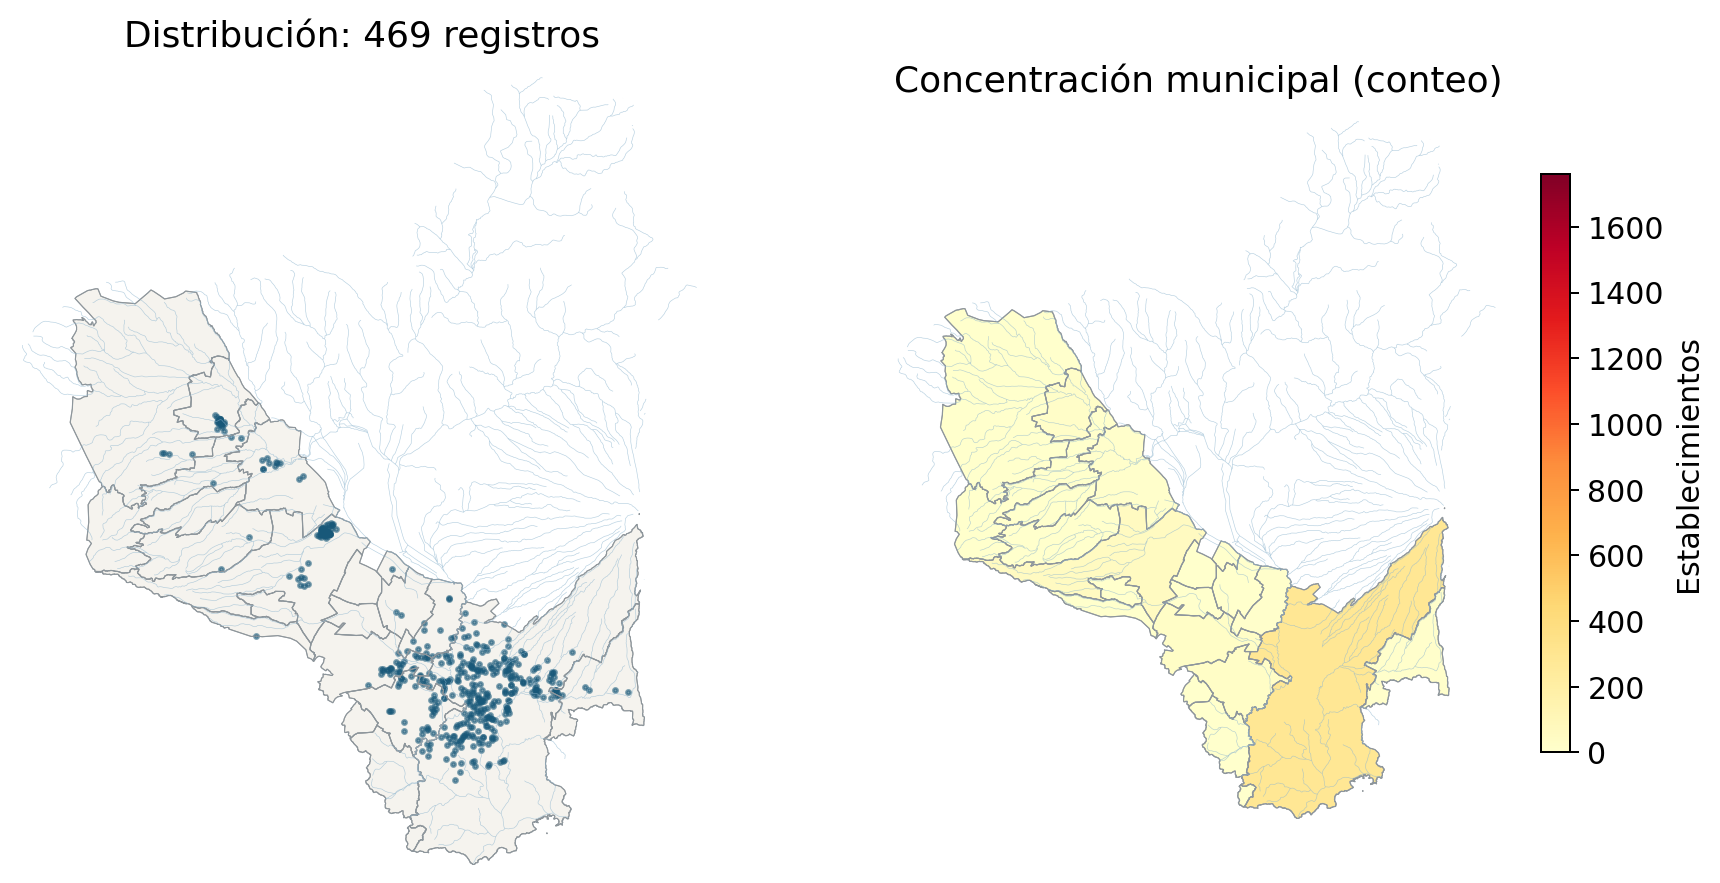
\includegraphics[width=.97\textwidth,height=.72\textheight,keepaspectratio]{direccion_imagenes/comparacion_modo_3.png}
\par\scriptsize Puntos a la izquierda; conteo por polígono a la derecha. Escala absoluta idéntica en las cinco modalidades.
\end{frame}
\begin{frame}{Distribución y concentración: Estricto + MH}
\centering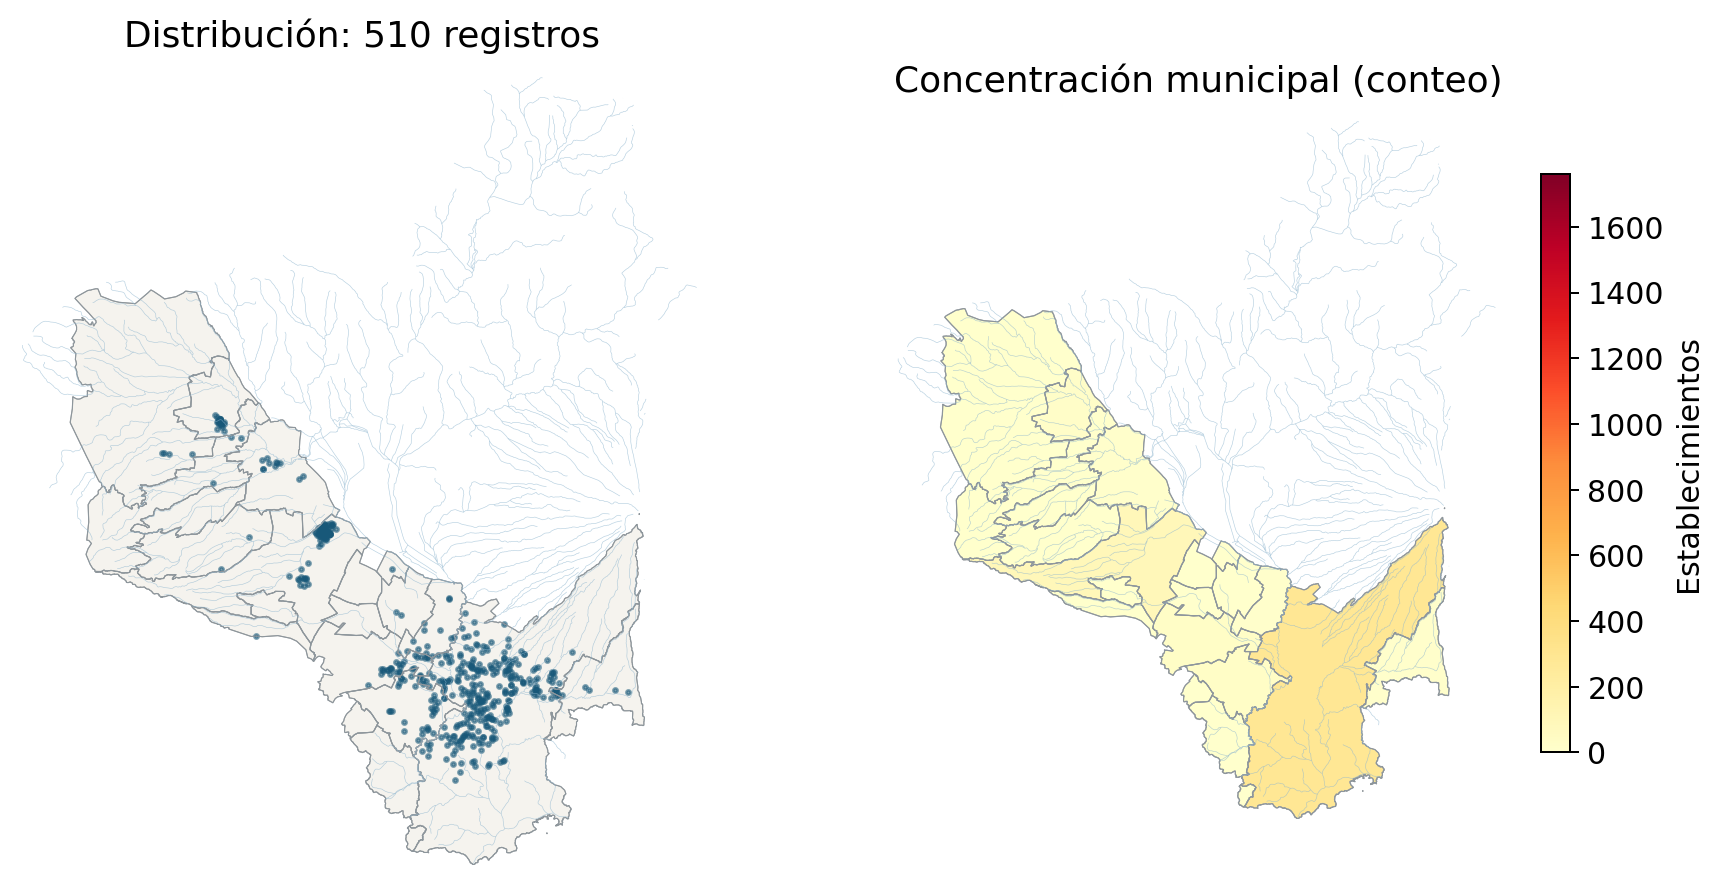
\includegraphics[width=.97\textwidth,height=.72\textheight,keepaspectratio]{direccion_imagenes/comparacion_modo_4.png}
\par\scriptsize Puntos a la izquierda; conteo por polígono a la derecha. Escala absoluta idéntica en las cinco modalidades.
\end{frame}
\begin{frame}{Posibles comerciales: definición del grupo}
\small
\begin{itemize}
\item Se seleccionan registros SCIAN exacto 812210 del amplio DENUE que no aparecen en estricto DENUE; se comparan identificadores dentro de la misma cuenca.
\item El grupo contiene 1,210 registros. Representa 72.1\% del universo amplio DENUE.
\item Son lavanderías sin señal adicional suficiente bajo la regla estricta. El grupo permite localizar dónde se concentra la diferencia entre escenarios.
\item La ausencia de señal industrial en nombre/razón social no demuestra operación comercial: también puede haber industriales poco descriptivas.
\item Se usan escenarios sin MH para aislar el cambio de regla; el mapa no clasifica automáticamente los registros MH como comerciales o industriales.
\end{itemize}
\end{frame}
\begin{frame}{Heatmap: dónde se concentran las posibles comerciales}
\centering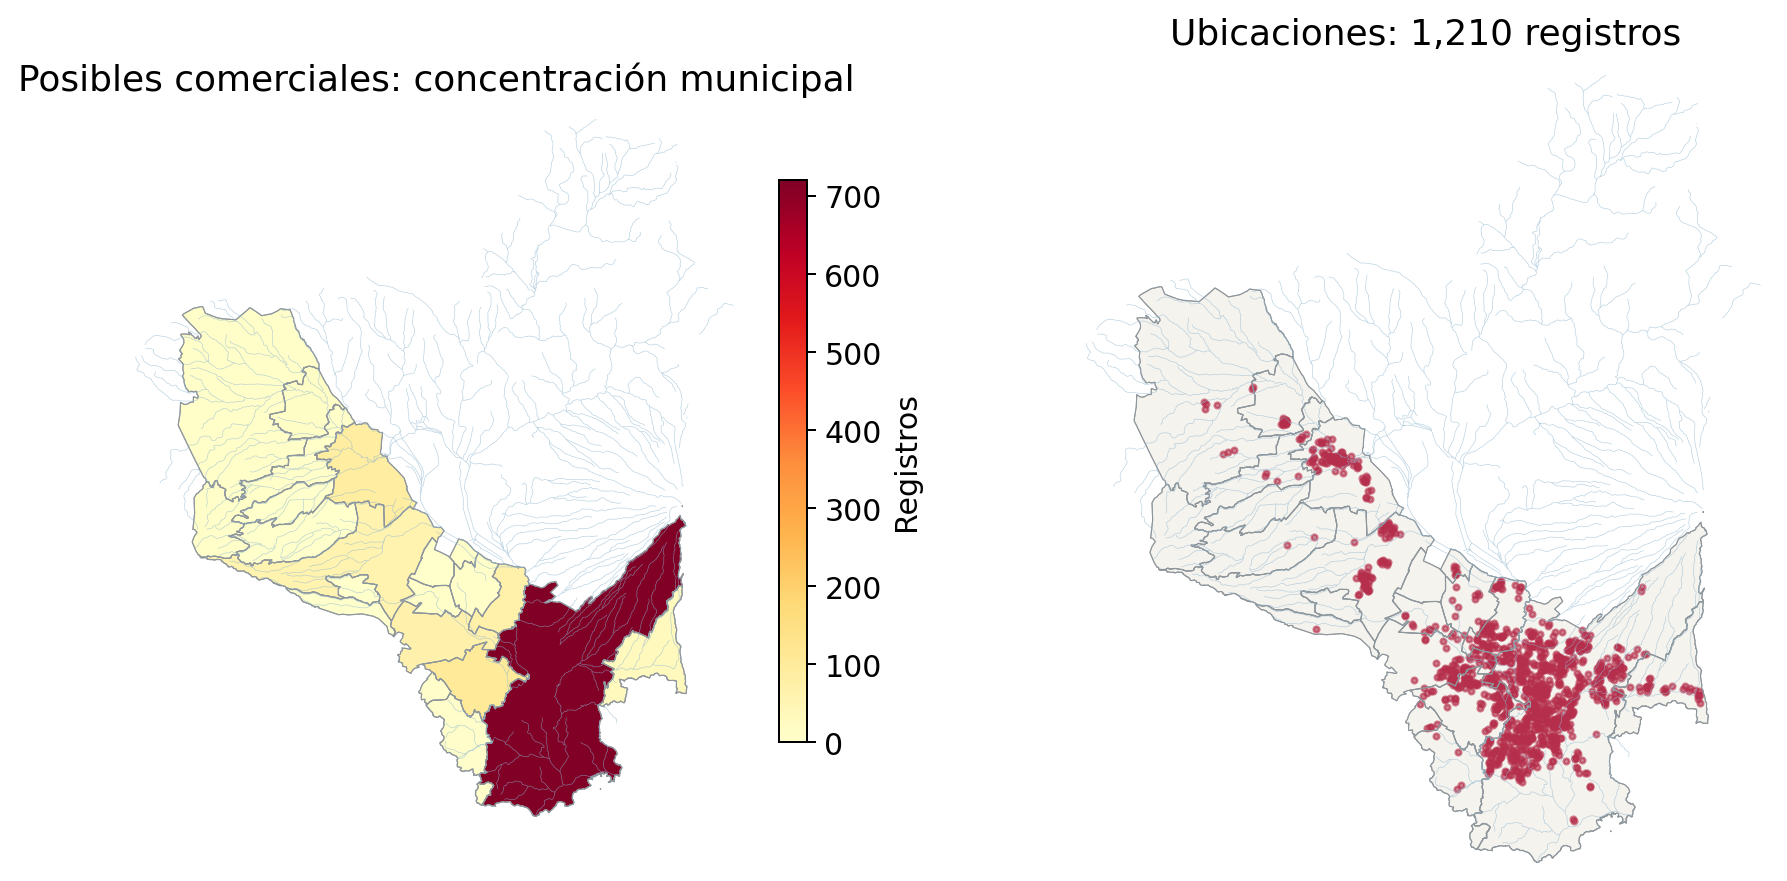
\includegraphics[width=.97\textwidth,height=.72\textheight,keepaspectratio]{direccion_imagenes/posibles_comerciales.png}
\par\scriptsize Aproximación por falta de señal adicional: SCIAN 812210 en amplio DENUE y ausente del estricto. Escala propia de este grupo.
\end{frame}
\begin{frame}{Posibles comerciales: municipios con más registros}
\centering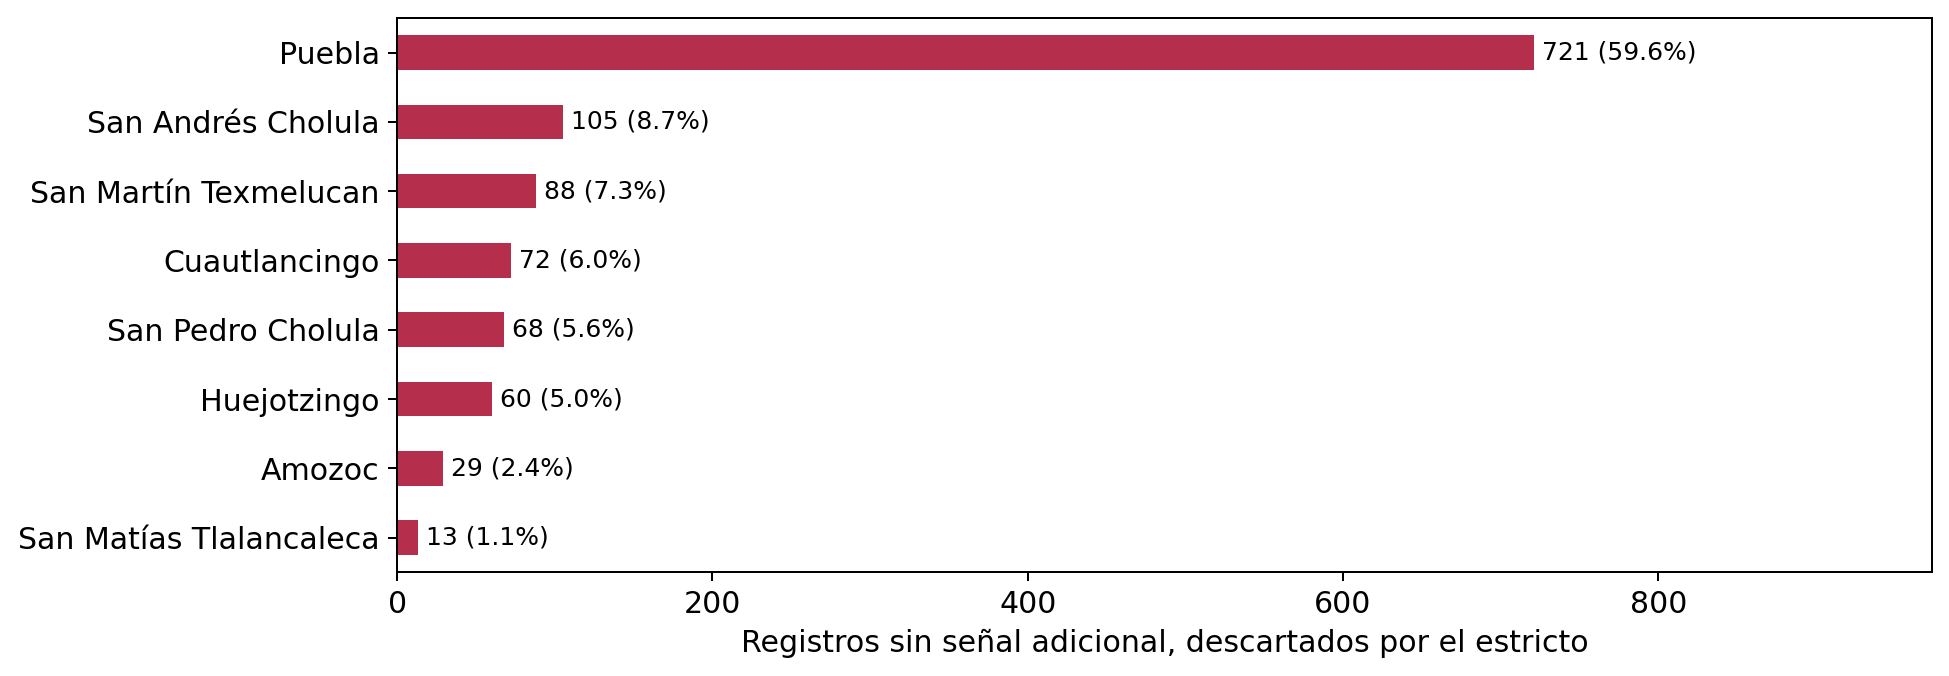
\includegraphics[width=.97\textwidth,height=.72\textheight,keepaspectratio]{direccion_imagenes/ranking_comerciales.png}
\par\scriptsize Conteo por municipio declarado, y porcentaje respecto al grupo de posibles comerciales; no es una verificación de tipo de operación.
\end{frame}
\begin{frame}{Qué aporta esta comparación a dirección}
\small
\begin{itemize}
\item Puebla concentra 721 de 1,210 posibles comerciales (59.6\%).
\item Comparar conteos absolutos muestra dónde se reduce más el inventario; comparar participación muestra cómo cambia el peso relativo de las zonas.
\item Los mapas individuales conservan escala común para que un municipio no parezca igualmente concentrado en escenarios con cantidades muy distintas.
\item MH añade cobertura localizada; la caída del amplio al estricto corresponde principalmente al criterio de lavanderías, no a establecimientos que desaparecen.
\item Las tablas y el listado de este grupo se guardan en docs/direccion\_imagenes para rastrear los registros que sostienen la comparación.
\end{itemize}
\end{frame}
\begin{frame}{Establecimientos pequeños: eje del marco territorial}
\small
\begin{itemize}
\item La comparación también separa los estratos DENUE 0 a 5 y 6 a 10 personas en las cinco modalidades.
\item La categoría de origen es 0 a 5; no se cambia a 1 a 5 porque el archivo no permite separar registros con cero personas.
\item Se utilizan como estratos operativos de establecimientos pequeños. El personal reportado no equivale por sí solo a una clasificación formal de microempresa ni mide producción.
\item Cada estrato tiene una escala de color común entre modalidades. Las escalas de 0 a 5 y 6 a 10 son distintas para hacer visible cada grupo.
\item Los registros con estrato vacío quedan fuera de ambos grupos y se mantienen como desconocidos. No se asignan automáticamente a los pequeños.
\end{itemize}
\end{frame}
\begin{frame}{Peso de los establecimientos pequeños en cada modalidad}\centering\scriptsize
\begin{tabular}{lllll}\toprule
Modalidad & 0 a 5 & \% universo & 6 a 10 & \% universo\\\midrule
Sectorial & 3332 & 83.1\% & 333 & 8.3\%\\
Amplio DENUE & 1595 & 95.0\% & 55 & 3.3\%\\
Amplio + MH & 1617 & 94.2\% & 61 & 3.6\%\\
Estricto DENUE & 419 & 89.3\% & 28 & 6.0\%\\
Estricto + MH & 441 & 86.5\% & 35 & 6.9\%\\
\bottomrule\end{tabular}
\par\medskip Denominador: todos los registros de cada modalidad dentro de cuenca, incluidos los de estrato desconocido.\end{frame}
\begin{frame}{Cinco modalidades: pequeños de 0 a 5 personas}
\centering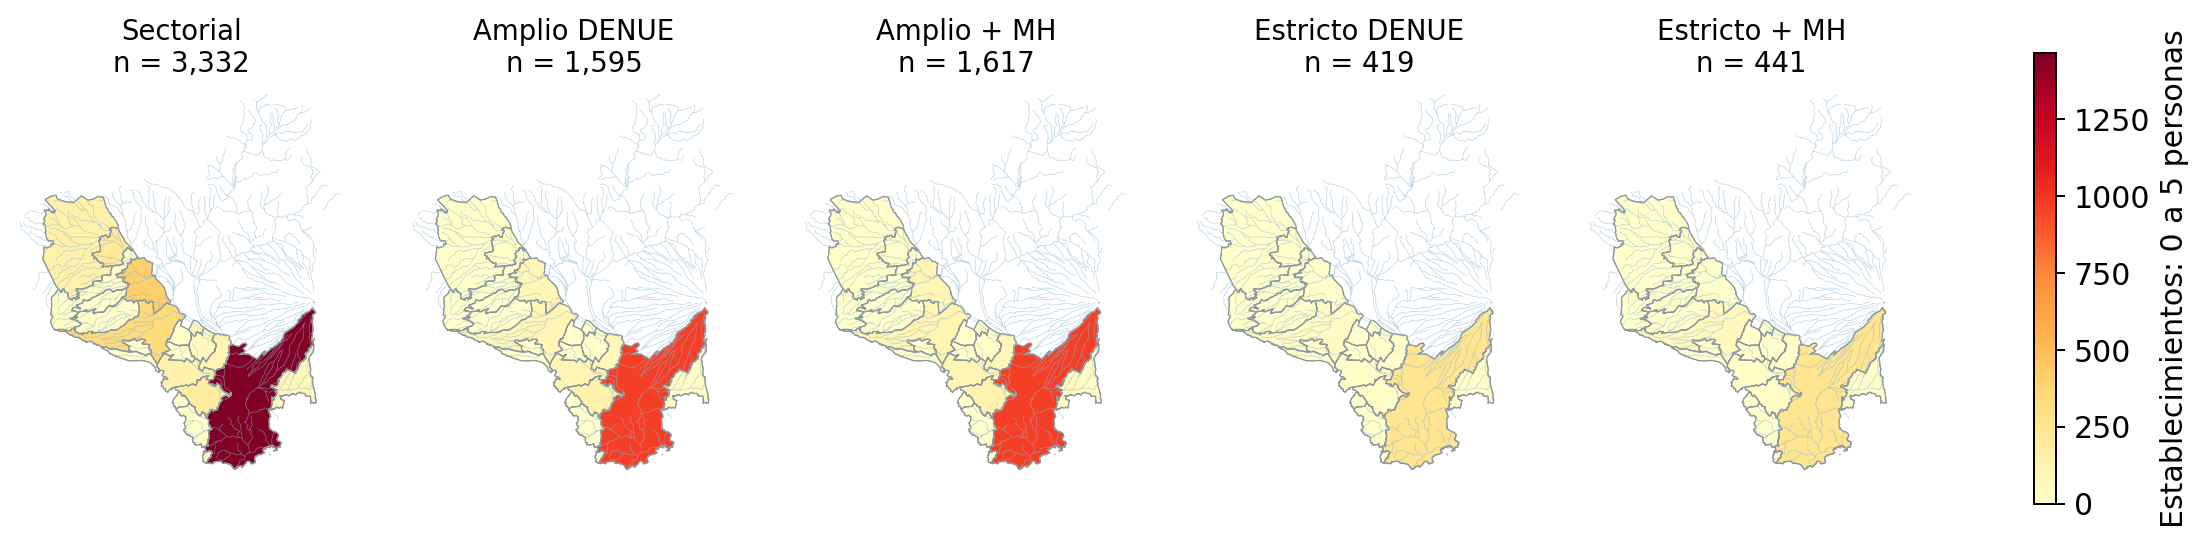
\includegraphics[width=.97\textwidth,height=.72\textheight,keepaspectratio]{direccion_imagenes/pequenas_panel_0.png}
\par\scriptsize Conteos espaciales con escala común dentro del estrato. Comparar solo mapas que tengan la misma barra de color.
\end{frame}
\begin{frame}{Sectorial: establecimientos de 0 a 5 personas}
\centering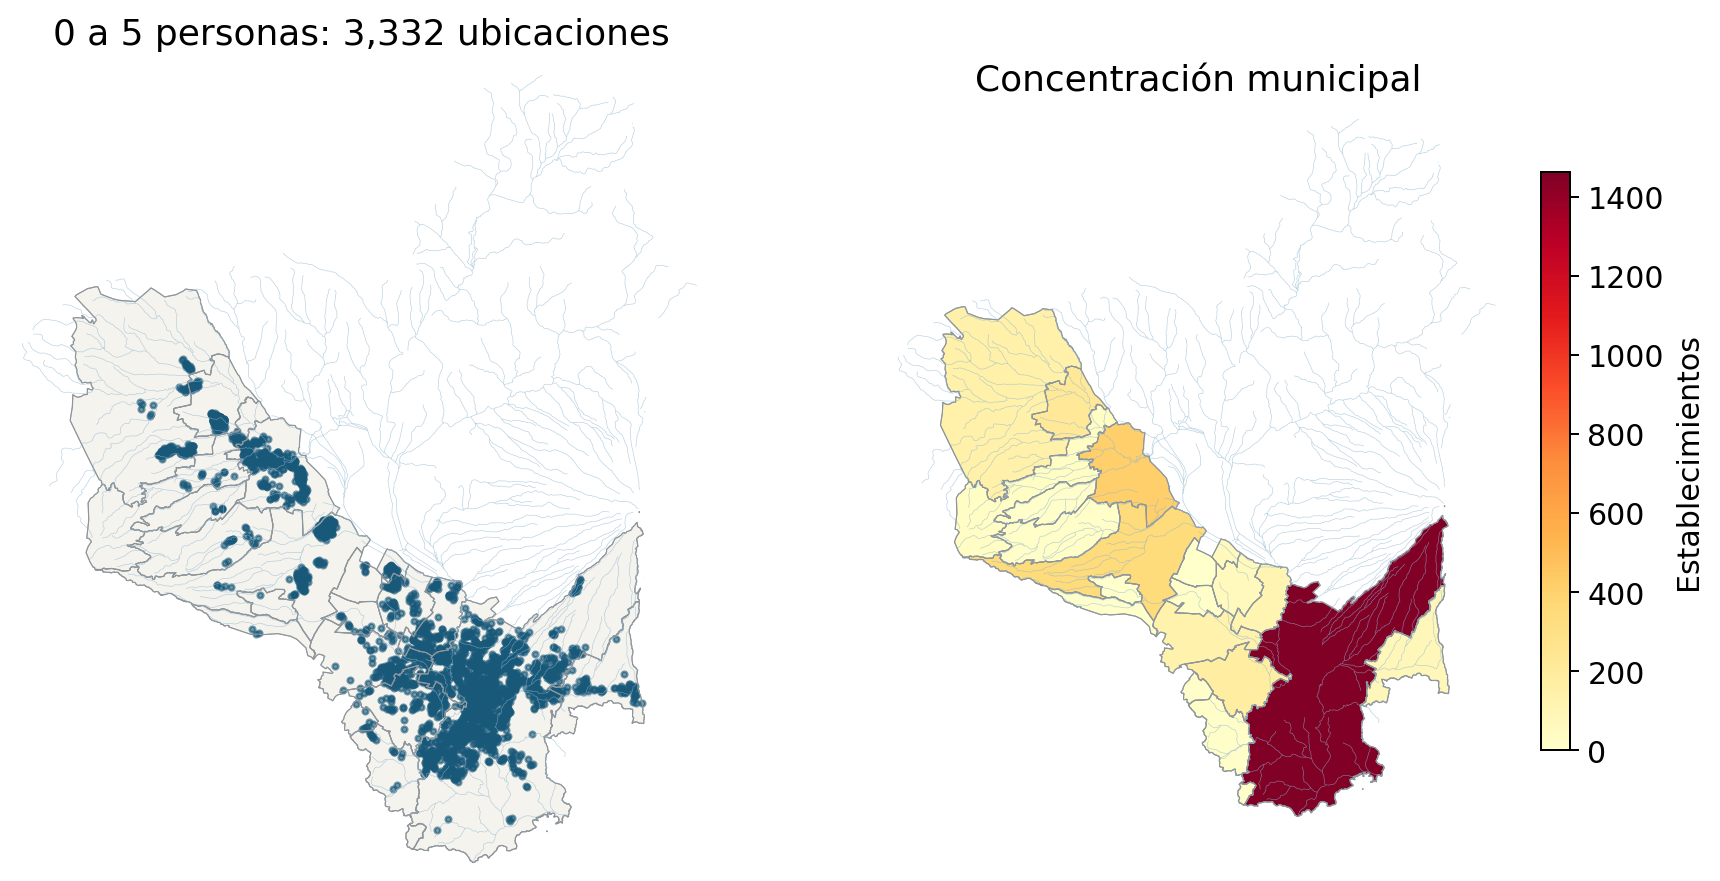
\includegraphics[width=.97\textwidth,height=.72\textheight,keepaspectratio]{direccion_imagenes/pequenas_0_modo_0.png}
\par\scriptsize Distribución puntual y concentración municipal del mismo grupo; campos de personal ocupado reportados por DENUE.
\end{frame}
\begin{frame}{Amplio DENUE: establecimientos de 0 a 5 personas}
\centering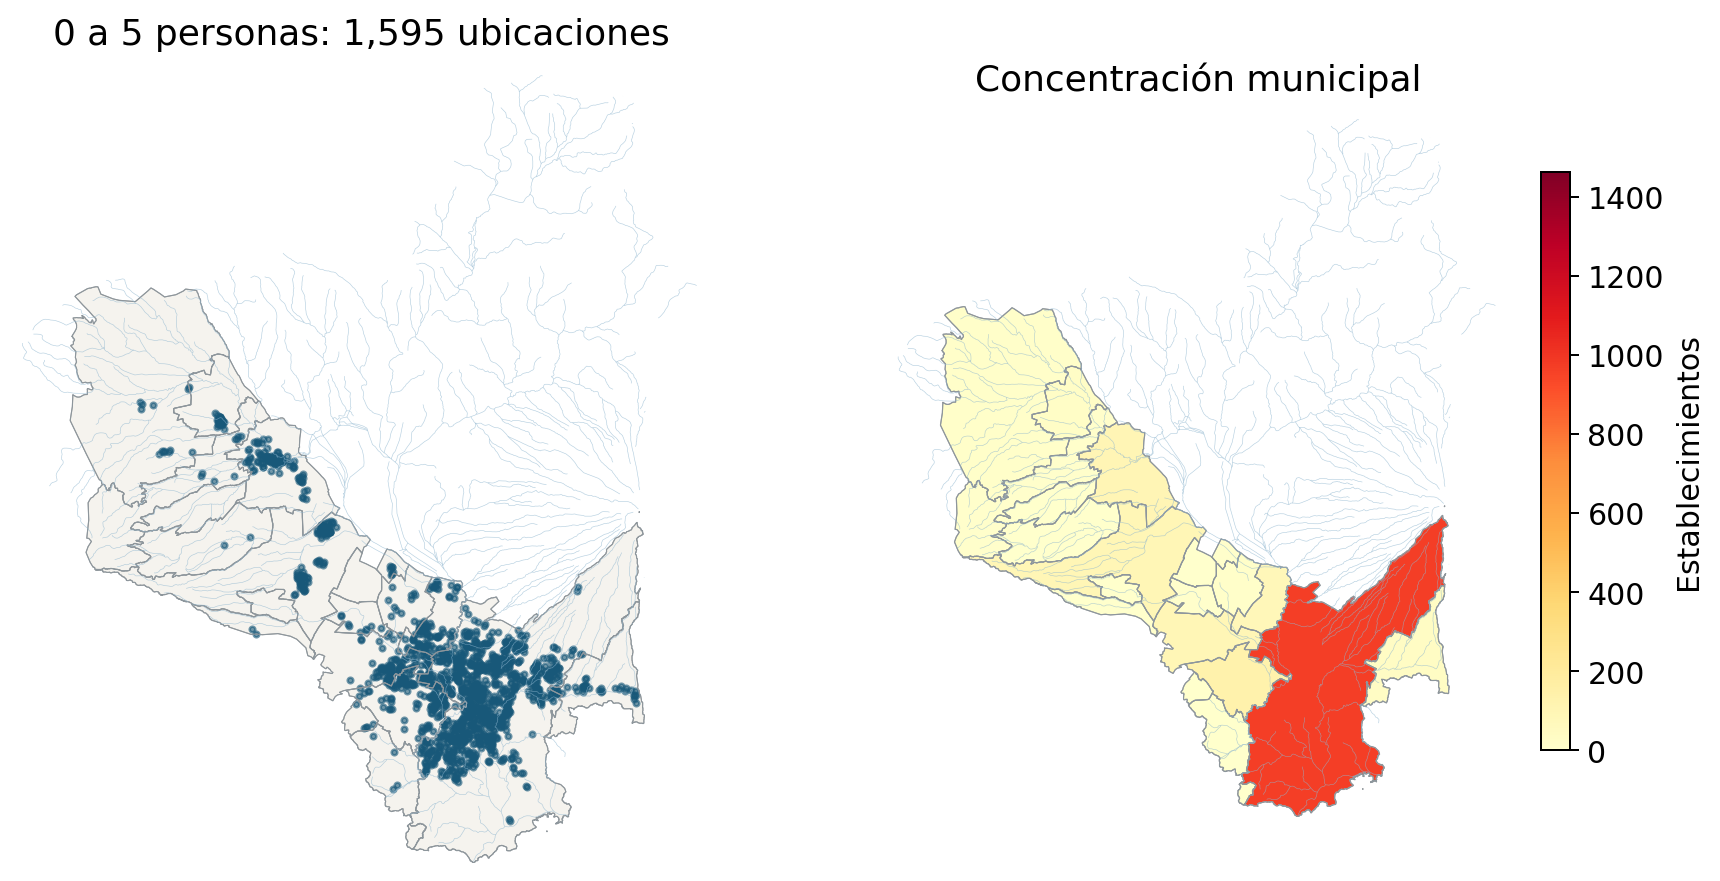
\includegraphics[width=.97\textwidth,height=.72\textheight,keepaspectratio]{direccion_imagenes/pequenas_0_modo_1.png}
\par\scriptsize Distribución puntual y concentración municipal del mismo grupo; campos de personal ocupado reportados por DENUE.
\end{frame}
\begin{frame}{Amplio + MH: establecimientos de 0 a 5 personas}
\centering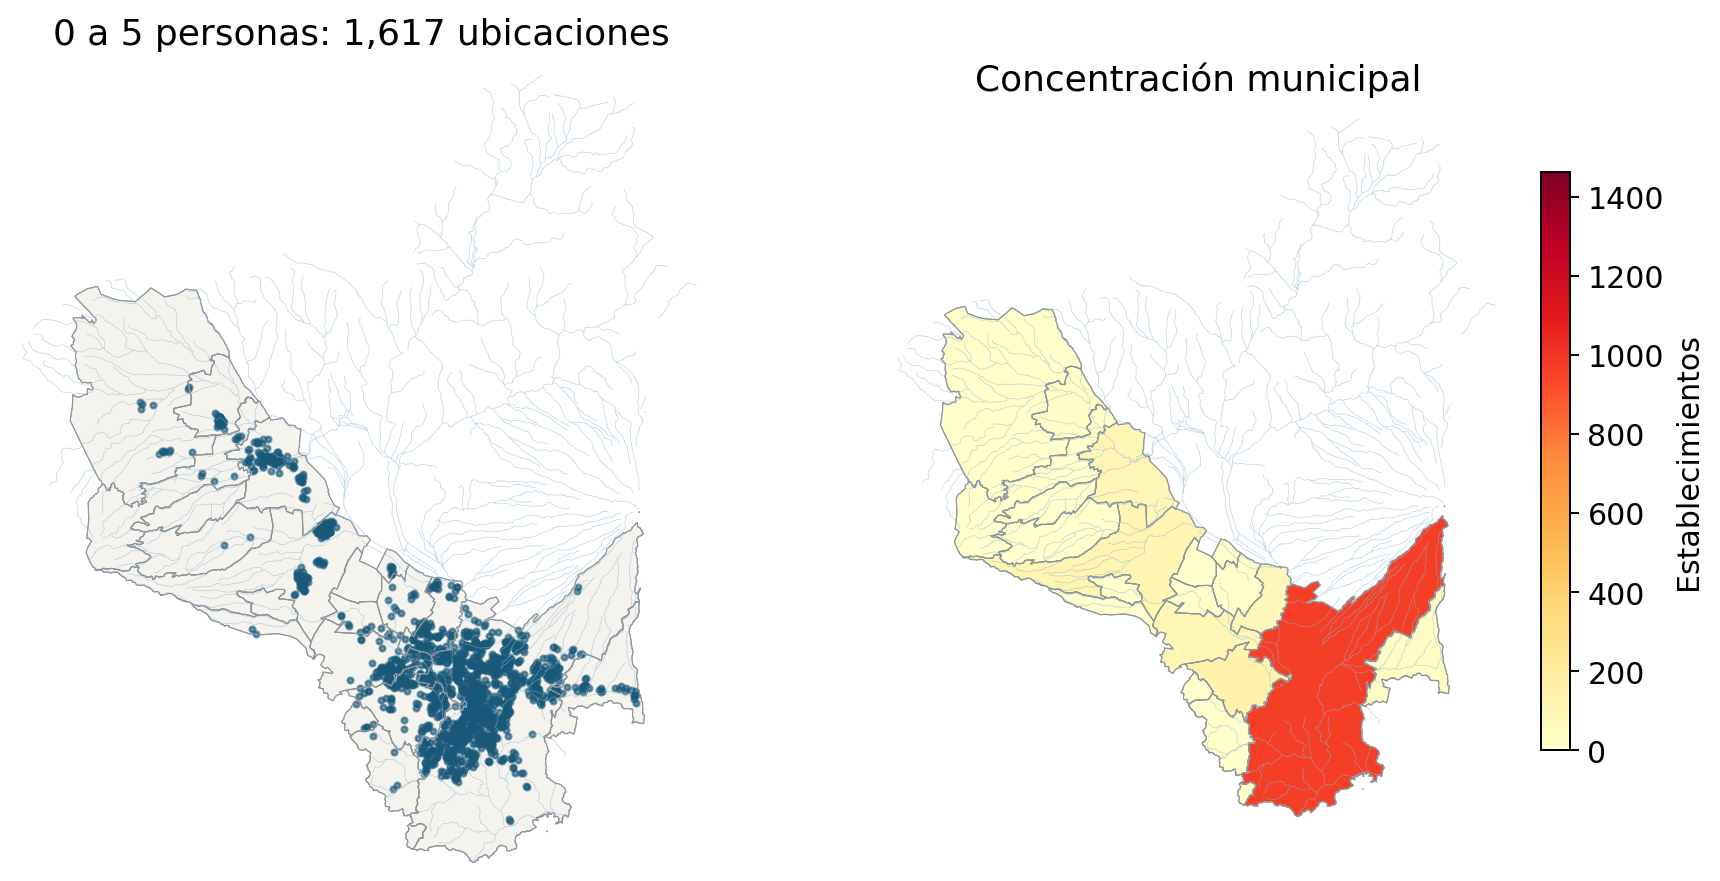
\includegraphics[width=.97\textwidth,height=.72\textheight,keepaspectratio]{direccion_imagenes/pequenas_0_modo_2.png}
\par\scriptsize Distribución puntual y concentración municipal del mismo grupo; campos de personal ocupado reportados por DENUE.
\end{frame}
\begin{frame}{Estricto DENUE: establecimientos de 0 a 5 personas}
\centering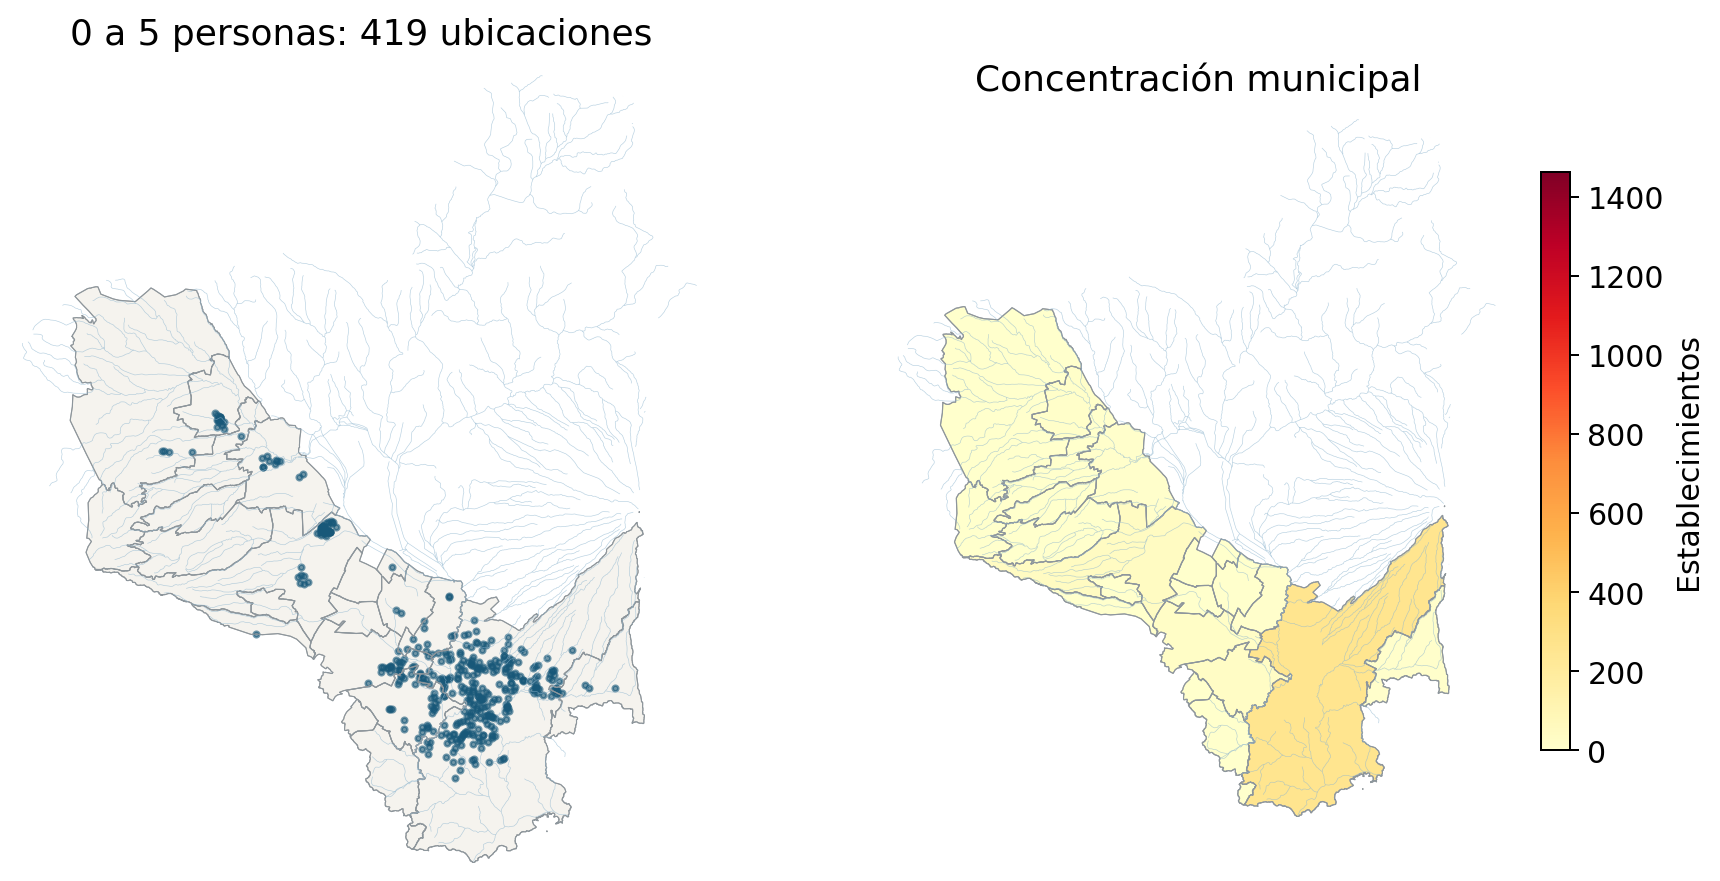
\includegraphics[width=.97\textwidth,height=.72\textheight,keepaspectratio]{direccion_imagenes/pequenas_0_modo_3.png}
\par\scriptsize Distribución puntual y concentración municipal del mismo grupo; campos de personal ocupado reportados por DENUE.
\end{frame}
\begin{frame}{Estricto + MH: establecimientos de 0 a 5 personas}
\centering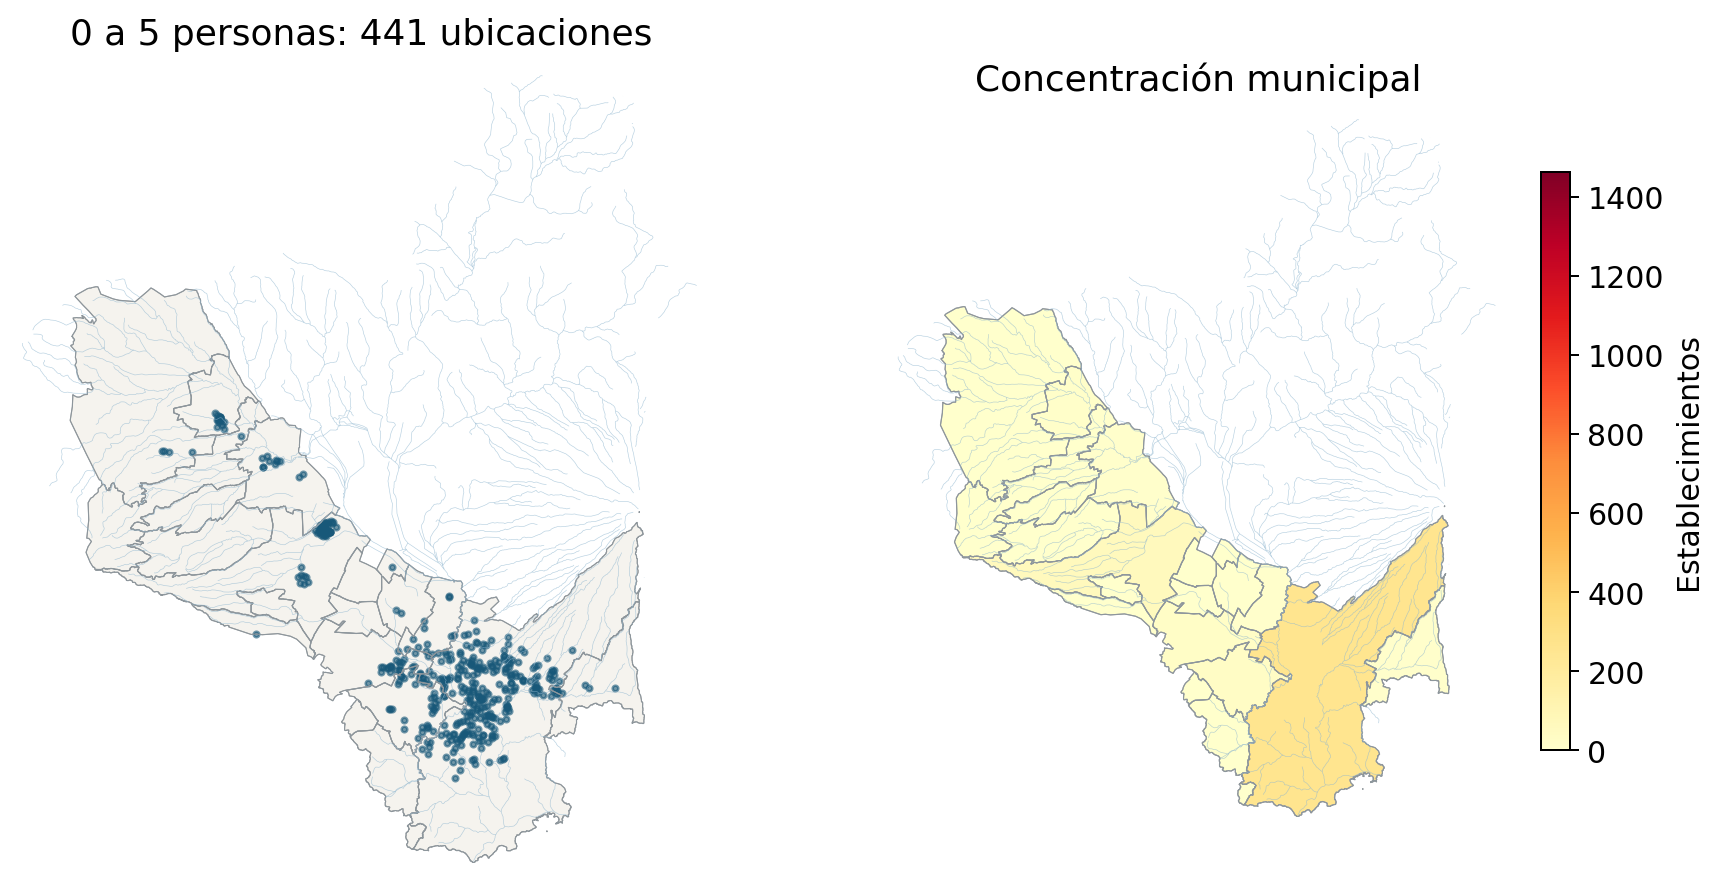
\includegraphics[width=.97\textwidth,height=.72\textheight,keepaspectratio]{direccion_imagenes/pequenas_0_modo_4.png}
\par\scriptsize Distribución puntual y concentración municipal del mismo grupo; campos de personal ocupado reportados por DENUE.
\end{frame}
\begin{frame}{Cinco modalidades: pequeños de 6 a 10 personas}
\centering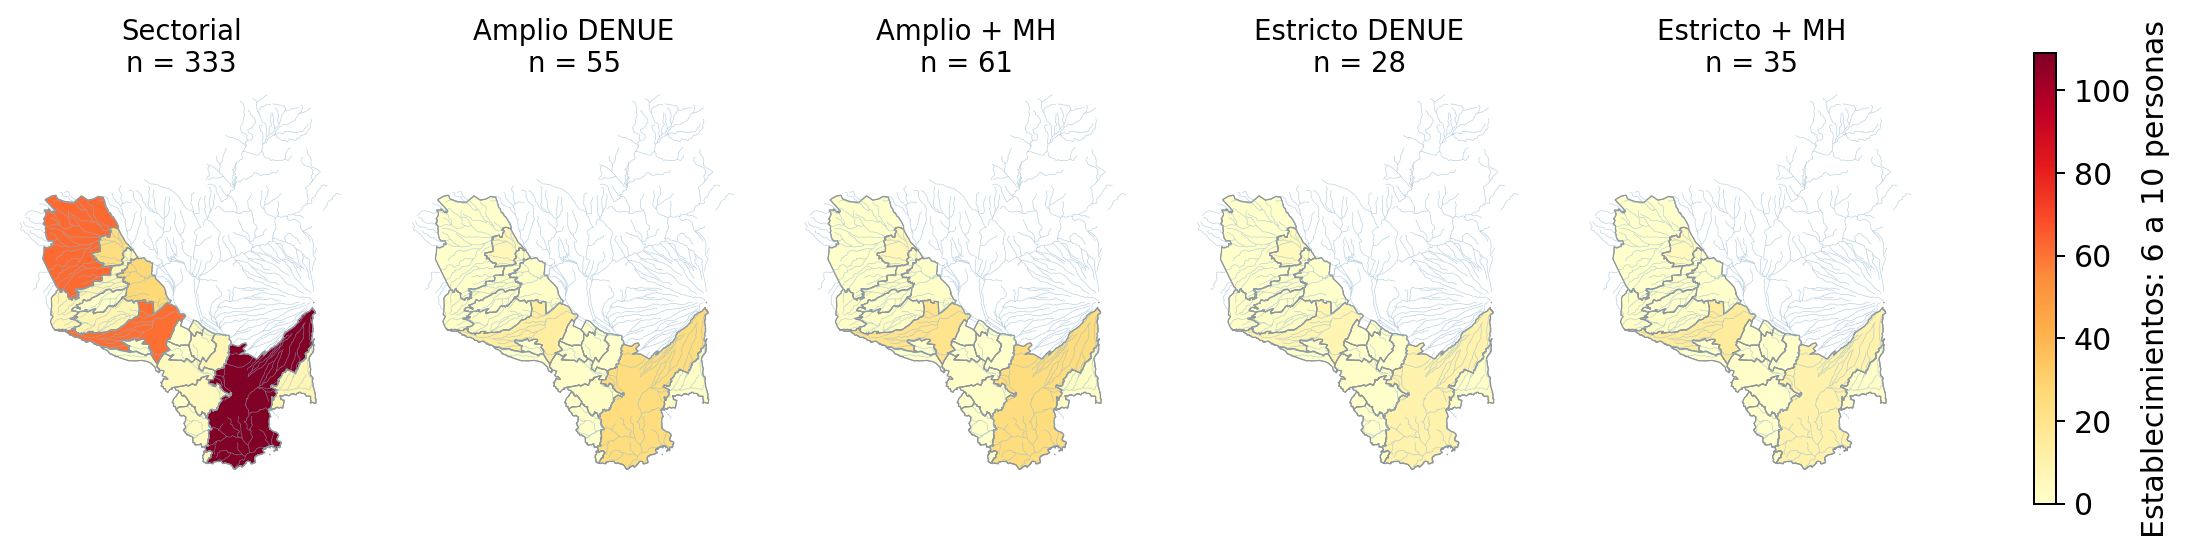
\includegraphics[width=.97\textwidth,height=.72\textheight,keepaspectratio]{direccion_imagenes/pequenas_panel_1.png}
\par\scriptsize Conteos espaciales con escala común dentro del estrato. Comparar solo mapas que tengan la misma barra de color.
\end{frame}
\begin{frame}{Sectorial: establecimientos de 6 a 10 personas}
\centering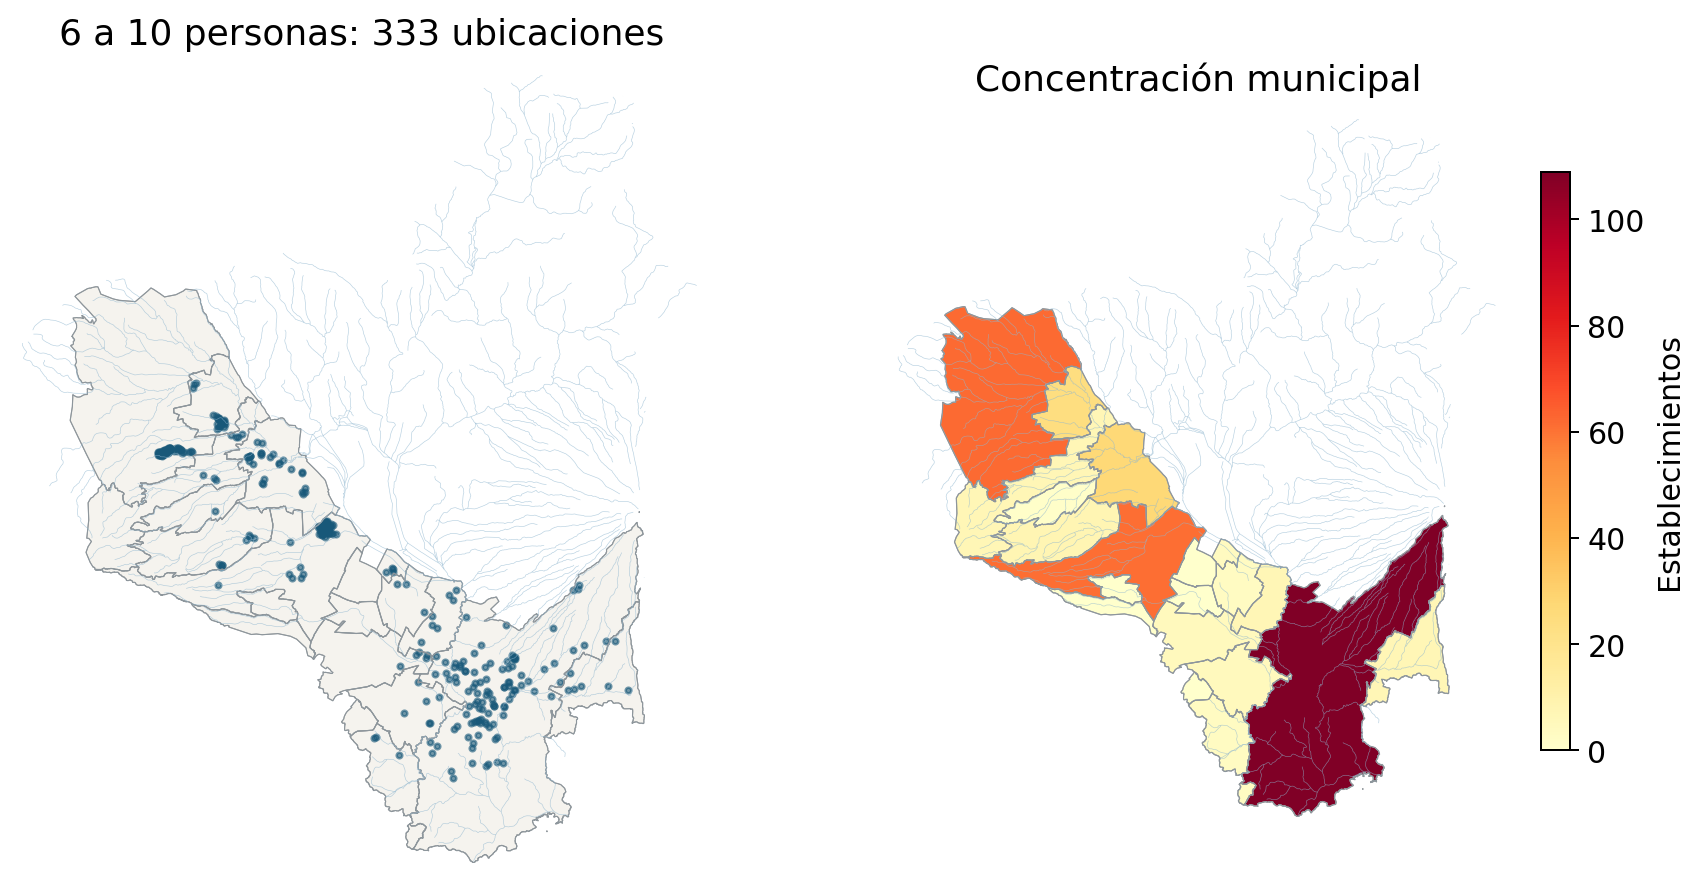
\includegraphics[width=.97\textwidth,height=.72\textheight,keepaspectratio]{direccion_imagenes/pequenas_1_modo_0.png}
\par\scriptsize Distribución puntual y concentración municipal del mismo grupo; campos de personal ocupado reportados por DENUE.
\end{frame}
\begin{frame}{Amplio DENUE: establecimientos de 6 a 10 personas}
\centering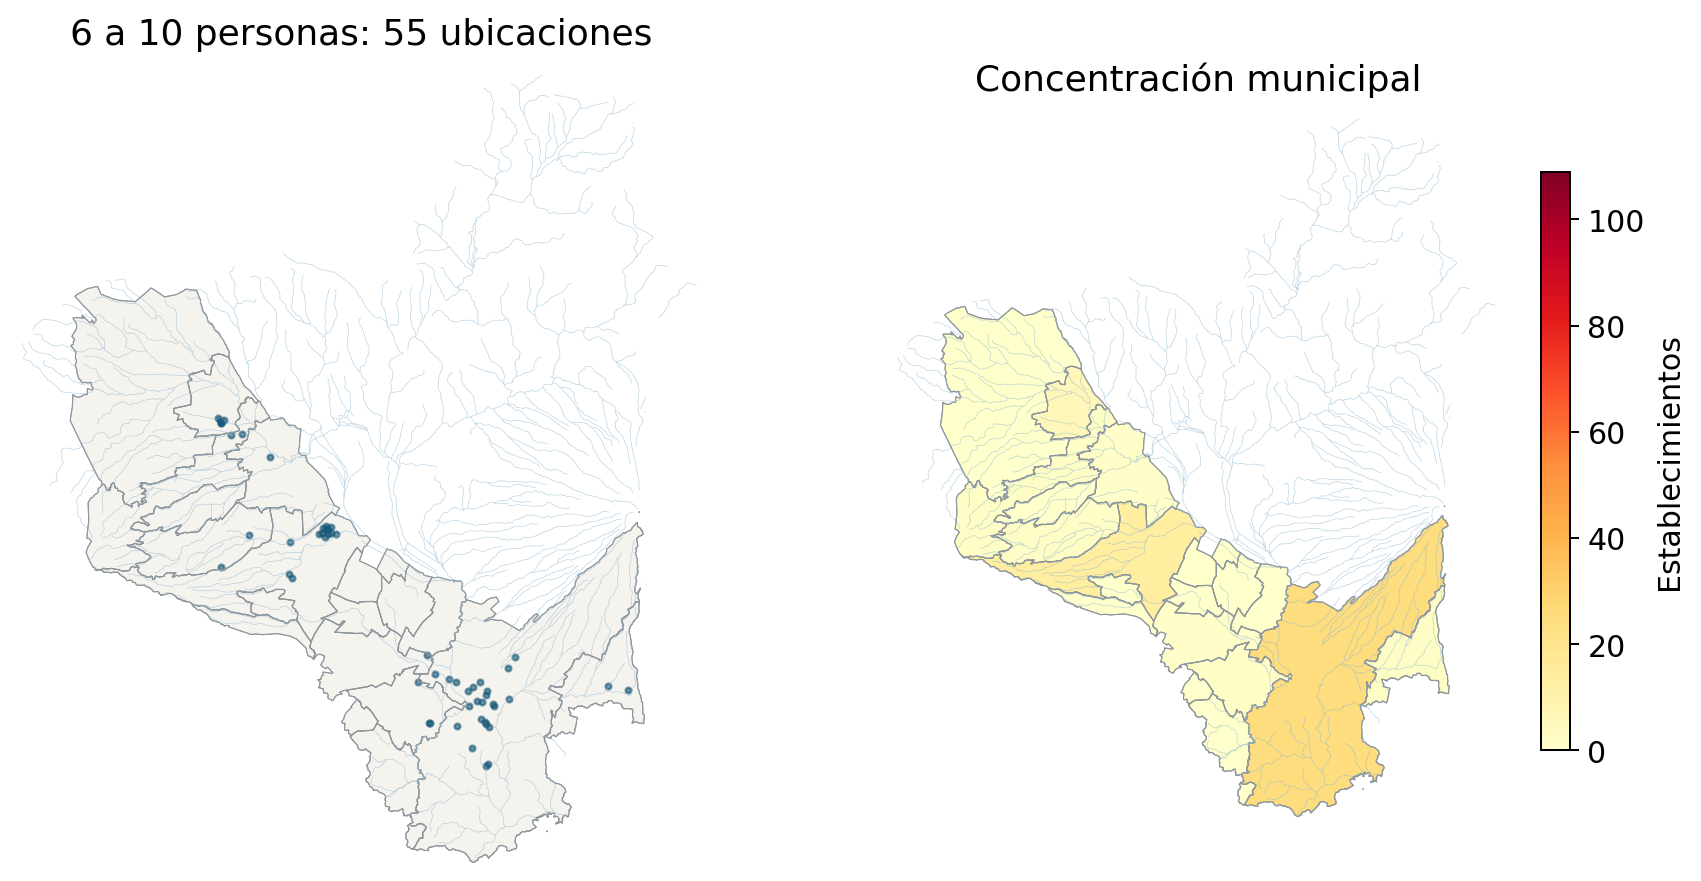
\includegraphics[width=.97\textwidth,height=.72\textheight,keepaspectratio]{direccion_imagenes/pequenas_1_modo_1.png}
\par\scriptsize Distribución puntual y concentración municipal del mismo grupo; campos de personal ocupado reportados por DENUE.
\end{frame}
\begin{frame}{Amplio + MH: establecimientos de 6 a 10 personas}
\centering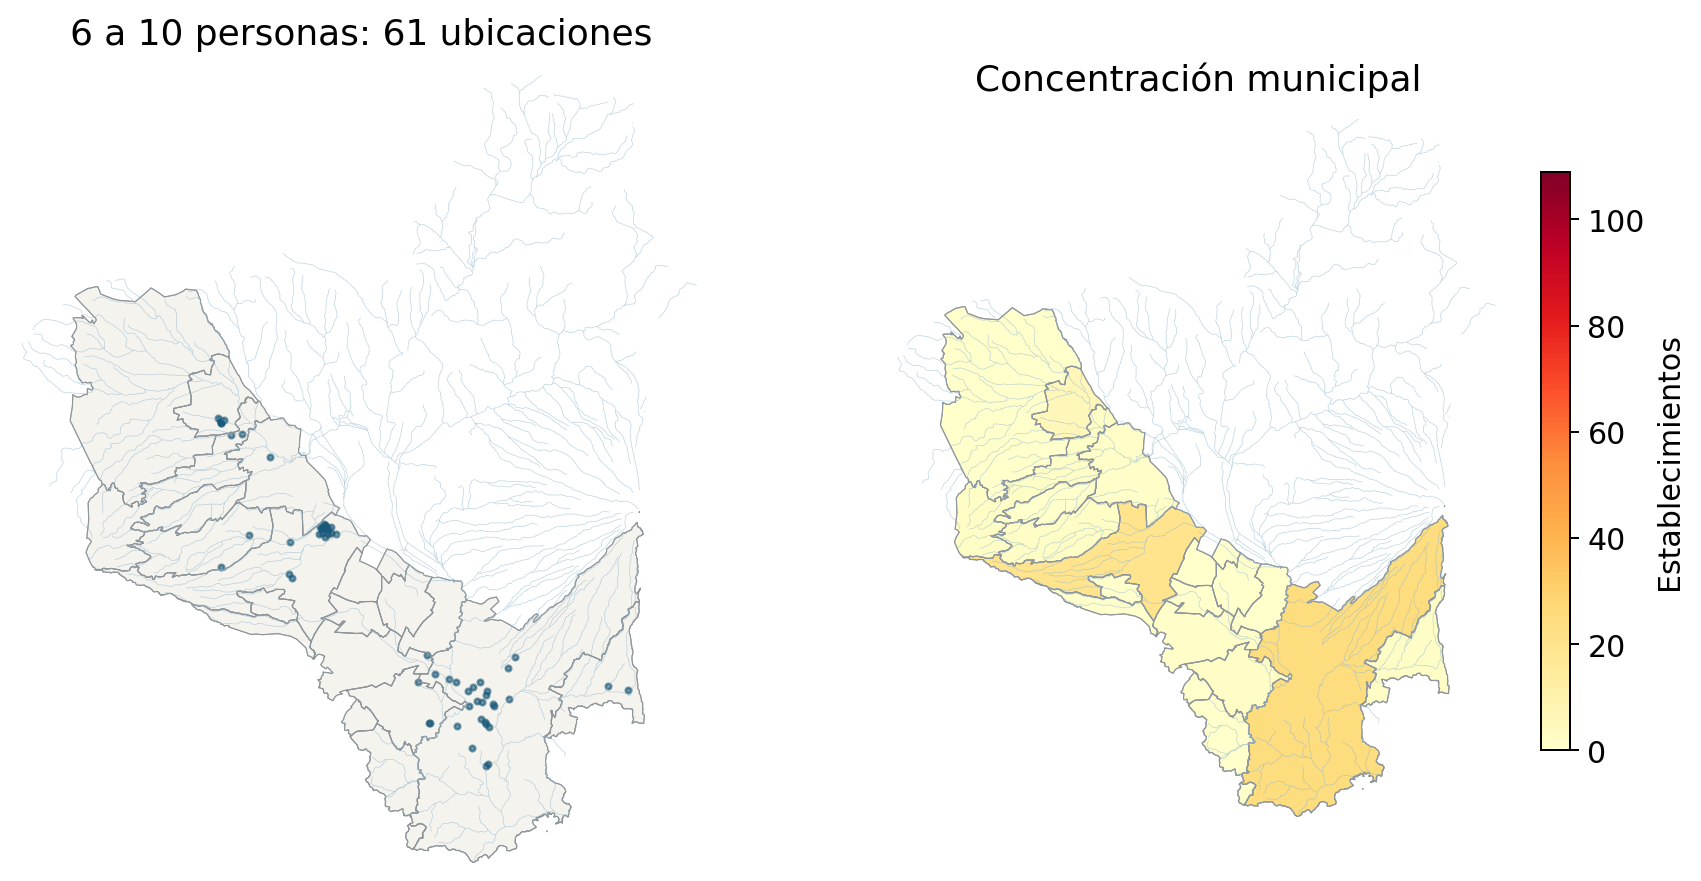
\includegraphics[width=.97\textwidth,height=.72\textheight,keepaspectratio]{direccion_imagenes/pequenas_1_modo_2.png}
\par\scriptsize Distribución puntual y concentración municipal del mismo grupo; campos de personal ocupado reportados por DENUE.
\end{frame}
\begin{frame}{Estricto DENUE: establecimientos de 6 a 10 personas}
\centering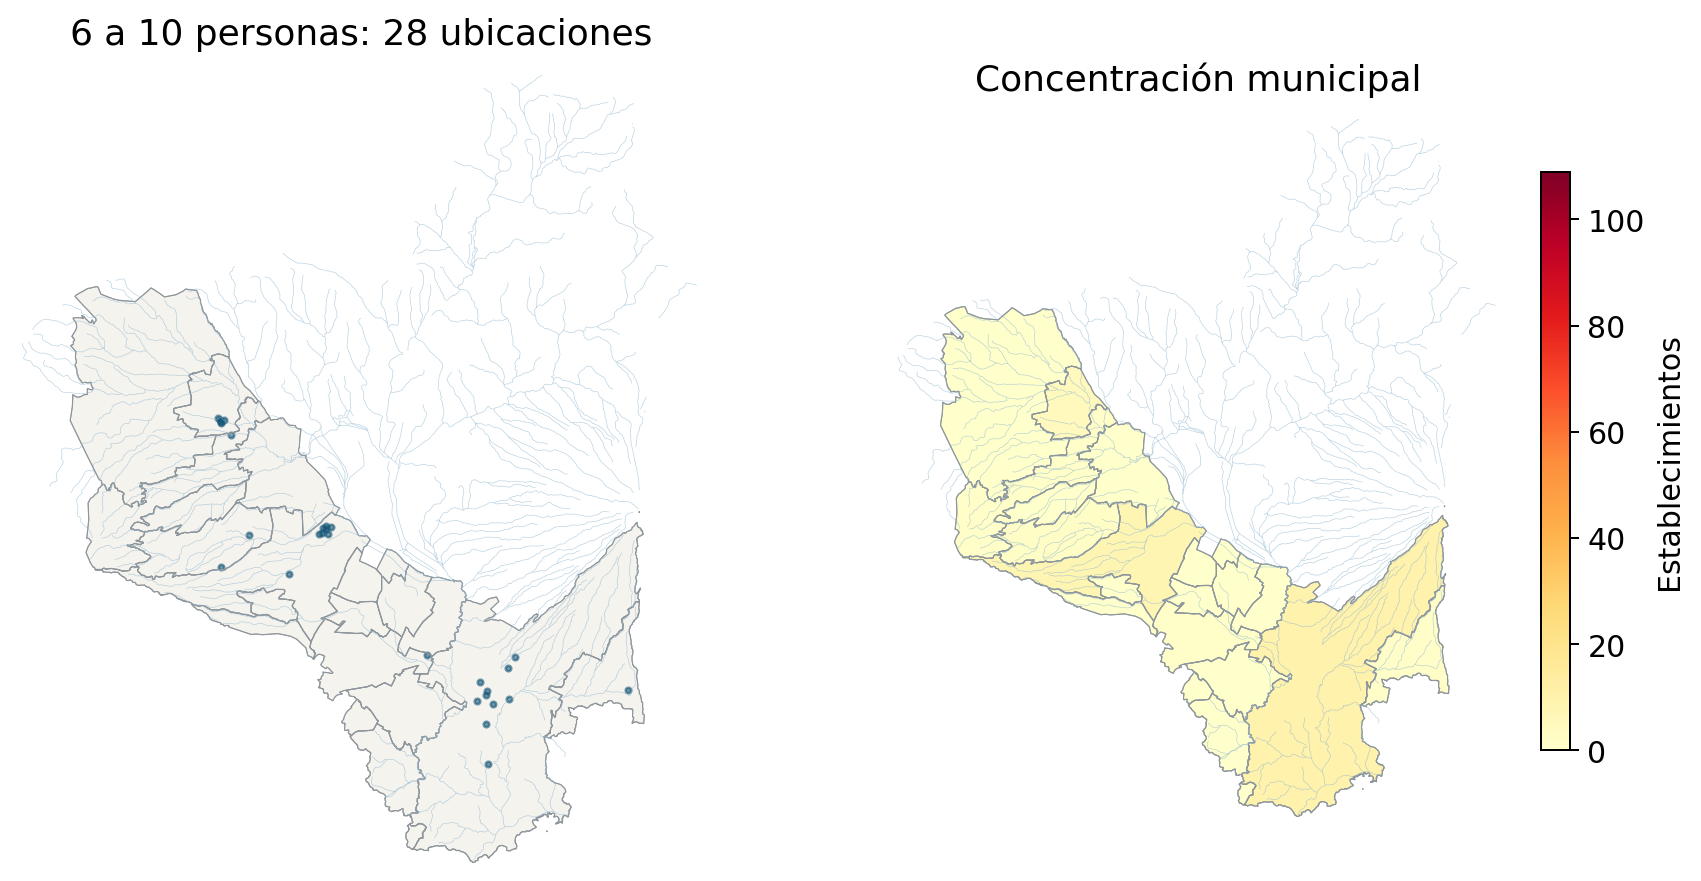
\includegraphics[width=.97\textwidth,height=.72\textheight,keepaspectratio]{direccion_imagenes/pequenas_1_modo_3.png}
\par\scriptsize Distribución puntual y concentración municipal del mismo grupo; campos de personal ocupado reportados por DENUE.
\end{frame}
\begin{frame}{Estricto + MH: establecimientos de 6 a 10 personas}
\centering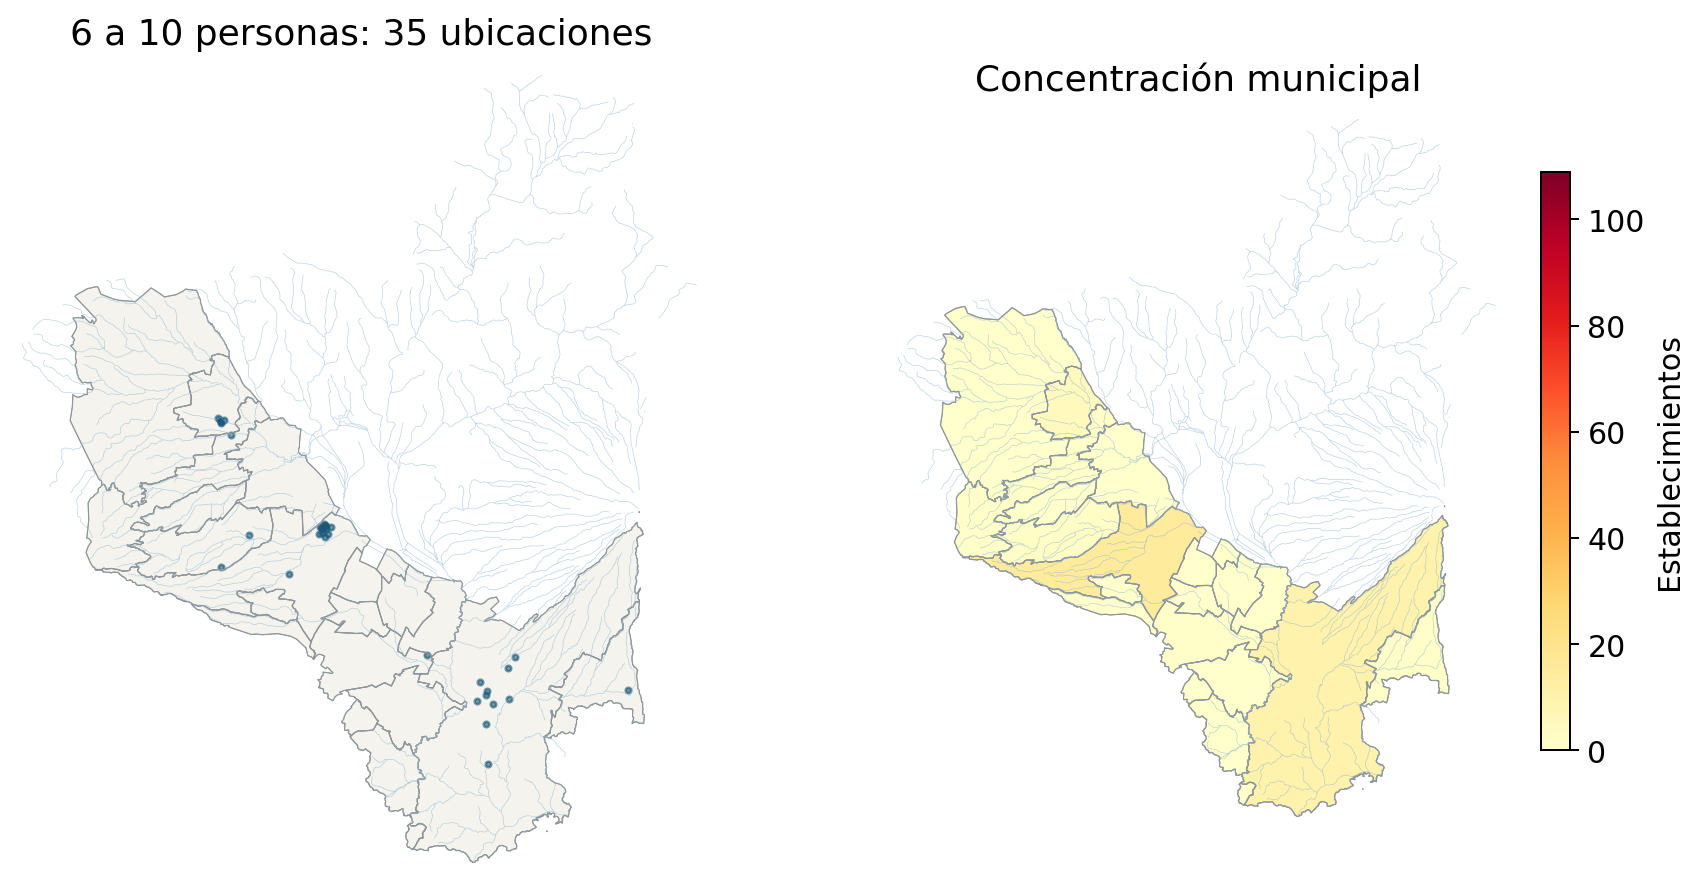
\includegraphics[width=.97\textwidth,height=.72\textheight,keepaspectratio]{direccion_imagenes/pequenas_1_modo_4.png}
\par\scriptsize Distribución puntual y concentración municipal del mismo grupo; campos de personal ocupado reportados por DENUE.
\end{frame}
\begin{frame}{Qué implica la concentración de establecimientos pequeños}
\small
\begin{itemize}
\item La predominancia de registros pequeños caracteriza una estructura territorial de numerosas unidades de baja ocupación reportada.
\item Los mapas permiten ubicar agrupaciones territoriales para orientar preguntas sobre servicios compartidos, procesos o vínculos productivos; esos vínculos requieren evidencia adicional.
\item Cambiar el filtro puede modificar tanto el número como la distribución de pequeños. La comparación por estrato evita atribuir todo el cambio a industrias grandes.
\item Un establecimiento con pocas personas puede operar procesos intensivos; el estrato no permite estimar agua utilizada o descarga.
\item Los registros MH sin personal reportado no se deben interpretar como grandes ni como pequeños. Su información faltante queda visible.
\end{itemize}
\end{frame}
\begin{frame}{Proceso 6A: preparación e integración MH}
\small
\begin{itemize}
\item Fuentes: capa final MH.shp de Xalmimilulco y base\_huejo(Hoja1) (1).csv de Huejotzingo.
\item Se conserva evidencia\_hidrica\_original y se añade fuente\_universo\_hidrico, fuente\_evidencia\_hidrica e id\_denue\_origen\_mh.
\item El código asigna SI a los registros asociados con MH y etiqueta MH\_TRABAJO\_CAMPO.
\item Esta asignación es una decisión del procedimiento; no acredita por sí sola qué proceso se comprobó.
\item 53 registros se procesan: 46 de Xalmimilulco y 7 de Huejotzingo; todos aparecen dentro del recorte de cuenca en las salidas actuales.
\end{itemize}
\end{frame}
\begin{frame}{Proceso 6B: correspondencia de Xalmimilulco}
\small
\begin{itemize}
\item La capa MH se transforma a EPSG:4326; se toma ID DENUE, eliminando .0 y tratando nulos como ID vacío.
\item Si ID ya está en universo hídrico: se conserva el registro DENUE, se cambia a SI y se añade procedencia MH; acción YA\_PRESENTE.
\item Si ID está en auditable pero fuera del hídrico: se recupera la fila DENUE y se asigna SI; acción AGREGADO\_DESDE\_DENUE.
\item Si no hay correspondencia en auditable: se crea registro suplementario MH\_XALMI\_..., con nombre y geometría MH; acción AGREGADO\_SUPLEMENTARIO.
\item Los suplementarios tienen sector REVISAR, evidencia original SIN\_REGISTRO\_DENUE\_2026 y campos DENUE no conocidos vacíos.
\item La búsqueda es contra auditable; SIN\_REGISTRO no acredita ausencia de cualquier registro en toda la base nacional DENUE.
\end{itemize}
\end{frame}
\begin{frame}{Proceso 6C: correspondencia de Huejotzingo}
\small
\begin{itemize}
\item El ID del CSV es local, no ID DENUE. Se excluyen nombres vacíos y se convierten coordenadas decimales o grados/minutos/segundos a latitud y longitud.
\item Se consideran candidatos auditables cuya localidad normalizada es Huejotzingo; se transforman a EPSG:32614.
\item Para cada fila MH se elige el candidato más cercano. Se calcula similitud de nombre con SequenceMatcher sobre texto normalizado.
\item Coincidencia = distancia menor o igual a 35 m y similitud mayor o igual a 0.45.
\item Si coincide: actualizar si ya está o recuperar desde DENUE. Si no: crear MH\_HUEJO\_... con geometría MH y campos administrativos vacíos.
\item Límite: se prueba solo el vecino más cercano; no se buscan otros vecinos si falla su nombre. Los umbrales no tienen validación estadística documentada.
\end{itemize}
\end{frame}
\begin{frame}{Proceso 6D: trazabilidad y controles MH}
\small
\begin{itemize}
\item La auditoría registra fuente, nombre, ID MH, ID de salida, acción, distancia y, para Huejotzingo, similitud de nombre.
\item Se concatenan recuperados y suplementarios; se rechazan ID de salida duplicados.
\item En las auditorías actuales no hay ID de salida repetidos. Esto no descarta duplicados físicos con ID distintos.
\item La evidencia original se conserva para evaluar cambios de clase; no se completa artificialmente el estrato de personal de suplementarios.
\item La cobertura MH es localizada: sus aportes no deben extrapolarse como tasa de omisión al resto del territorio.
\end{itemize}
\end{frame}
\begin{frame}{Qué cambia MH en cada modalidad}\centering\scriptsize
\begin{tabular}{lllll}\toprule
Modalidad & Ya presentes & Recuperados DENUE & Suplementarios & Total MH\\\midrule
Amplio + MH & 15 & 31 & 7 & 53\\
Estricto + MH & 12 & 34 & 7 & 53\\
\bottomrule\end{tabular}
\par\medskip Incrementos netos: 38 y 41. En ambos, SI pasa de 41 a 91: MH reclasifica casos previos además de incorporar registros.\end{frame}
\begin{frame}{Cómo leer los 91 registros SI}
\small
\begin{itemize}
\item En amplio + MH y estricto + MH hay 53 SI con fuente MH\_TRABAJO\_CAMPO y 38 SI con fuente REGLAS\_DENUE.
\item Antes de MH hay 41 SI automáticos. Tres de ellos cambian de fuente al estar también en MH.
\item Por eso 41 + 53 no se debe sumar como registros independientes: las fuentes se superponen.
\item La procedencia de la evidencia debe acompañar cada conteo SI para distinguir reglas automáticas de información MH.
\end{itemize}
\end{frame}
\begin{frame}{Proceso 7: recorte real de cuenca}
\small
\begin{itemize}
\item Se lee el polígono de cuenca y se transforma a EPSG:4326.
\item Se retienen puntos que intersectan la primera geometría del archivo de cuenca; un punto en el borde puede quedar incluido.
\item Se exportan por separado universo municipal y universo dentro de cuenca; no deben confundirse sus conteos.
\item El flujo cartográfico recorta red hidrográfica y polígonos municipales por la cuenca.
\item Los mapas de cada municipio usan puntos within del polígono recortado: un punto en el límite puede tratarse distinto del recorte intersects.
\item La operación usa geometry.iloc[0]; si cambia la estructura del archivo de cuenca, debe comprobarse que esa geometría represente el área completa.
\end{itemize}
\end{frame}
\begin{frame}{Distribución: misma extensión, dos escenarios}
\centering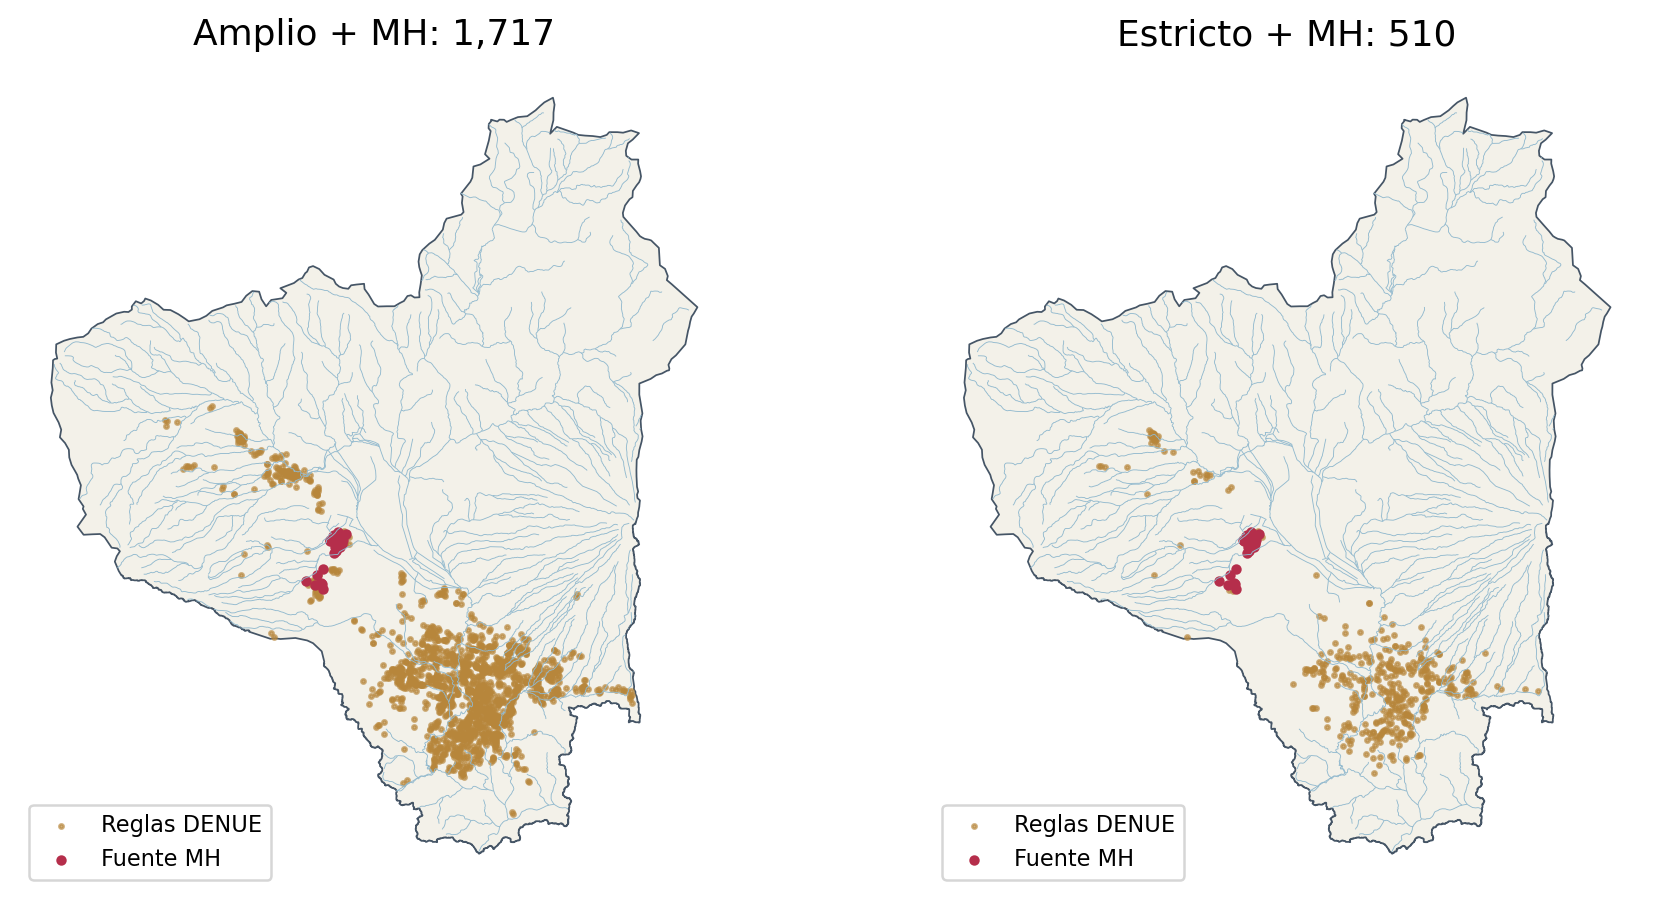
\includegraphics[width=.97\textwidth,height=.72\textheight,keepaspectratio]{direccion_imagenes/mapas_comparables.png}
\par\scriptsize Comparación elaborada desde capas GPKG, con la misma extensión y simbología. La fuente MH se distingue en rojo.
\end{frame}
\begin{frame}{Dónde cambia la concentración municipal}
\centering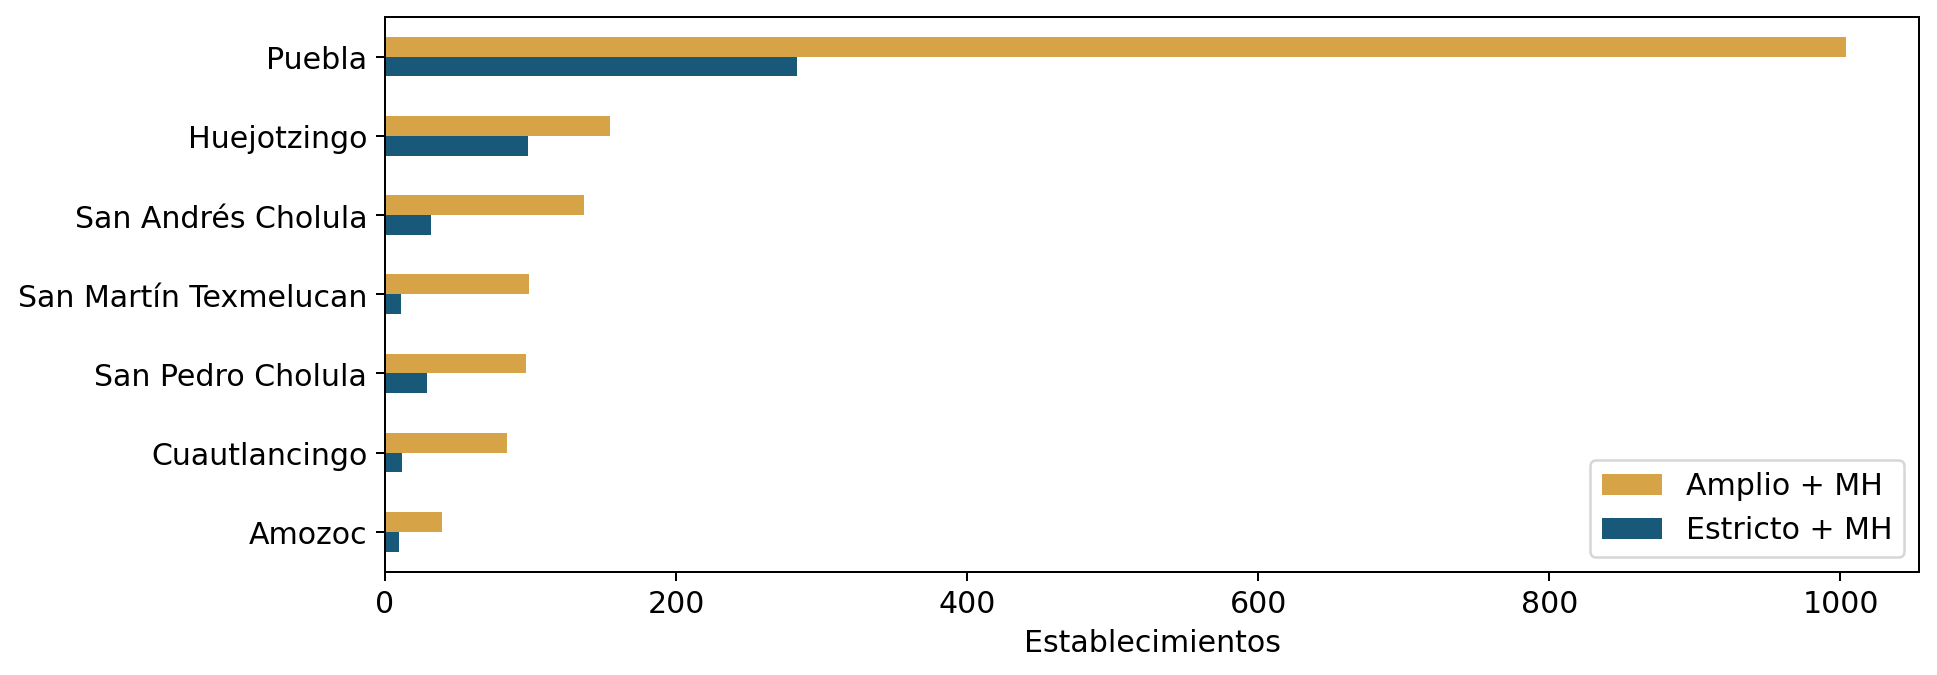
\includegraphics[width=.97\textwidth,height=.72\textheight,keepaspectratio]{direccion_imagenes/municipios.png}
\par\scriptsize Conteos por municipio declarado en el registro, dentro del recorte de cuenca; no son tasas ni volúmenes de descarga.
\end{frame}
\begin{frame}{Hallazgo territorial y efecto de cobertura}
\small
\begin{itemize}
\item Con MH, Puebla tiene 1,004 registros en amplio y 283 en estricto; Huejotzingo tiene 155 y 98, respectivamente.
\item La participación de Huejotzingo pasa de 9.0\% a 19.2\% al cambiar amplio + MH por estricto + MH.
\item Los 41 registros añadidos por MH al estricto están en el municipio de Huejotzingo: su conteo pasa de 57 a 98.
\item El orden y peso territorial dependen del filtro y de la cobertura de fuentes; no deben interpretarse automáticamente como diferencias de presión ambiental.
\item El marco permite contextualizar las zonas de interés dentro del inventario territorial.
\end{itemize}
\end{frame}
\begin{frame}{Proceso 8: tamaño y agregación espacial}
\small
\begin{itemize}
\item Tamaño = estrato de personal ocupado de DENUE; no se convierte a empleo exacto ni a capacidad productiva.
\item En estricto + MH, 441 de 510 registros (86.5\%) reportan 0 a 5 personas; 35 (6.9\%) reportan 6 a 10.
\item Los registros sin estrato se mantienen como desconocidos; no se asignan a microestablecimientos.
\item Los conteos municipales describen cantidad de registros. Las localidades se agregan por municipio + localidad.
\item Sin polígonos de localidad, el mapa usa centros medios de sus establecimientos: no son límites oficiales ni áreas de influencia.
\item El tamaño administrativo no permite concluir si una lavandería es comercial o industrial.
\end{itemize}
\end{frame}
\begin{frame}{Concentración por localidad: estricto con MH}
\centering
\includegraphics[width=.97\textwidth,height=.72\textheight,keepaspectratio]{../outputs/cuenca_alto_atoyac_puebla_estricto_mh/maps/png/06_conteo_localidad.png}
\par\scriptsize Agregaciones puntuales; el centro medio puede desplazarse al cambiar el conjunto de establecimientos.
\end{frame}
\begin{frame}{Proceso 9: distancia a la red hidrográfica}
\small
\begin{itemize}
\item Se reproyectan puntos y red hidrográfica recortada a EPSG:32614 (UTM 14N).
\item Se une la geometría de la red y se calcula distancia mínima geométrica de cada punto, en metros.
\item Se agrupa con pd.cut: hasta 250 m; más de 250 hasta 500 m; más de 500 hasta 1,000 m; más de 1,000 hasta 2,000 m; más de 2,000 m.
\item Los intervalos de salida llevan etiquetas 0-250, 250-500, 500-1,000, 1-2 km y >2 km; los límites superiores se incluyen.
\item Es proximidad cartográfica a la red proporcionada. No incorpora drenaje, tuberías, topografía, ruta del efluente o punto real de descarga.
\item Sirve para contextualizar o priorizar información adicional; no mide conexión hidráulica ni causalidad ambiental.
\end{itemize}
\end{frame}
\begin{frame}{Proximidad en el escenario de priorización}
\centering
\includegraphics[width=.97\textwidth,height=.72\textheight,keepaspectratio]{../outputs/cuenca_alto_atoyac_puebla_estricto_mh/maps/png/03_establecimientos_distancia_rio.png}
\par\scriptsize Distancia euclidiana mínima a la red incluida y recortada por cuenca; interpretar con las limitaciones de la diapositiva anterior.
\end{frame}
\begin{frame}{Ventajas y observaciones: sectorial y amplio}
\small
\begin{itemize}
\item Sectorial: ofrece contexto económico y distribución de la cadena textil; incluye actividades sin señales húmedas. Es el denominador contextual, no un universo de lavanderías industriales.
\item Amplio DENUE: cubre lavanderías de nombres poco informativos; 1,586 de sus 1,679 registros tienen SCIAN 812210.
\item El amplio evita descartar por falta de vocabulario, pero no separa lavanderías comerciales e industriales.
\item Amplio + MH: añade evidencia localizada y registros omitidos; mejora información en zonas cubiertas sin resolver la ambigüedad en todo el territorio.
\item Estas modalidades son útiles para contexto y sensibilidad, no para inferir cantidad de industrias contaminantes.
\end{itemize}
\end{frame}
\begin{frame}{Ventajas y observaciones: estricto}
\small
\begin{itemize}
\item Estricto DENUE: baja de 1,679 a 469 candidatos; conserva 376 SCIAN 812210. La reducción es operativa, no validación de exactitud.
\item Puede perder casos industriales por nombres genéricos; puede retener casos comerciales por señales generales como ropa o tintorería.
\item Estricto + MH: 510 candidatos; recupera 41 registros por información localizada. Es una base razonable de priorización acompañada de procedencia.
\item El catálogo contiene términos amplios, por ejemplo acabado y lavado de ropa; la categoría SI exige interpretar qué evidencia aportó el término.
\item No existen estimaciones documentadas de sensibilidad o precisión del clasificador. Ninguna modalidad constituye el conteo real verificado.
\end{itemize}
\end{frame}
\begin{frame}{Antecedente local y comparación histórica}
\small
\begin{itemize}
\item El flujo 100\_main trabaja Huejotzingo y Santa Ana Xalmimilulco con descarga local del 04/09/2026: primero recorta localidad y después aplica las reglas.
\item Exporta candidatos, SI y SI + REVISAR; recupera geometrías desde la capa original por identificador y genera figuras locales.
\item El flujo 07 compara por ID normalizado contra universos legacy: coincidencias, solo actual, solo histórico y diagnóstico probable de ausencias.
\item Los históricos y los actuales pueden diferir en fuente, fecha, cobertura, registros sin ID y definición de candidato.
\item Su función es explicar evolución del procedimiento; no se interpretan diferencias como apertura o cierre de establecimientos sin evidencia adicional.
\end{itemize}
\end{frame}
\begin{frame}{Desajustes documentales que dirección debe conocer}
\small
\begin{itemize}
\item La presentación anterior afirma usar descripción SCIAN para exclusiones; el texto\_filtro actual solo concatena nombre y razón social.
\item Algunos títulos anteriores dicen confirmados para todos los SI. Aquí se distingue SI por reglas de la procedencia MH.
\item El campo SIN\_REGISTRO\_DENUE\_2026 en suplementarios refiere a ausencia de correspondencia en el conjunto auditable utilizado.
\item Las tablas actuales son las cifras de esta presentación; corregir títulos no cambia ni valida retrospectivamente los criterios.
\item Esta entrega no modifica el clasificador ni las fuentes: deja visibles sus decisiones y límites para acordar mejoras.
\end{itemize}
\end{frame}
\begin{frame}{Revisión viable para una zona extensa}
\small
\begin{itemize}
\item Mantener clasificación automática reproducible para todo el territorio y conservar la incertidumbre por registro.
\item Concentrar la revisión en correspondencias MH dudosas y casos que afecten una decisión concreta.
\item No condicionar el avance a una auditoría manual exhaustiva de los 4,010 registros sectoriales.
\item Si se requiere evaluar desempeño del filtro, diseñar después una revisión acotada por grupos: retenidos, descartados y tipos de evidencia.
\item Esa revisión serviría para conocer errores del método; no se presenta aquí como realizada ni como validación ya disponible.
\end{itemize}
\end{frame}
\begin{frame}{Decisiones propuestas para dirección}
\small
\begin{itemize}
\item Adoptar estricto + MH como escenario de priorización de candidatos y amplio como contraste de cobertura.
\item Conservar el sectorial como contexto económico; reportar siempre territorio, modalidad y fuente junto a cada cifra.
\item Definir qué se observó en MH antes de utilizar el término verificado.
\item Priorizar la actualización de información en registros cuya incertidumbre afecte decisiones del proyecto.
\item El entregable territorial queda como marco de relevancia y selección de preguntas; la fase siguiente aporta evidencia específica de operación.
\end{itemize}
\end{frame}
\begin{frame}{Trazabilidad y reproducción de las cinco modalidades}
\small
\begin{itemize}
\item Flujo actual: python scripts/101\_main\_cuenca\_puebla.py (amplio + MH).
\item Agregar --sin-mh para amplio DENUE; --estricto para estricto + MH; --estricto --sin-mh para estricto DENUE.
\item Agregar --todos-scian para escenario sectorial; esa opción omite MH.
\item Reproducción de esta entrega: python scripts/102\_presentacion\_direccion.py. Lee las salidas existentes y compila el PDF.
\item Una nueva corrida territorial regenera HTML/PNG del directorio correspondiente. Para conservar versiones, archivar previamente salidas y catálogo.
\item Fecha de preparación: 17/09/2026. Fuentes: archivos locales del proyecto; no se incorporaron datos externos.
\end{itemize}
\end{frame}
\begin{frame}{Archivos y campos para auditar un resultado}
\small
\begin{itemize}
\item 02\_scian.py: prefijos; 03\_text\_filter.py + giro\_textil.csv: señales; 04\_desiciones\_preliminares.py: decisiones y precedencia.
\item 101\_main\_cuenca\_puebla.py: carga, municipios, modalidades y cuenca; 10\_integrar\_mh.py: correspondencias y suplementarios.
\item 08\_mapas\_cuenca\_puebla.py: distancias, agregaciones y mapas; 09\_presentacion\_cuenca\_puebla.py: presentaciones anteriores.
\item En cada carpeta outputs/cuenca\_alto\_atoyac\_puebla*: tablas de ejecución, auditable estatal, universo sectorial, hídrico previo a MH, final, dentro de cuenca y distancias.
\item Auditar por d\_llave, señales, coincide\_filtro\_scian/texto, sector\_textil, evidencia\_hidrica/original, fuentes e ID de origen MH.
\item El archivo auditoria\_integracion\_mh.csv explica cada acción de integración; inventario\_mapas.csv localiza PNG y HTML.
\end{itemize}
\end{frame}
\begin{frame}{Anexo: municipios solicitados (1/2)}
\small
\begin{itemize}
\item Amozoc; Calpan; Chiautzingo; Chignahuapan
\item Coronango; Cuautinchán; Cuautlancingo; Domingo Arenas
\item Huejotzingo; Ixtacamaxtitlán; Juan C. Bonilla; Ocoyucan
\item Puebla
\end{itemize}
\end{frame}
\begin{frame}{Anexo: municipios solicitados (2/2)}
\small
\begin{itemize}
\item San Andrés Cholula; San Felipe Teotlalcingo; San Gregorio Atzompa; San Jerónimo Tecuanipan
\item San Martín Texmelucan; San Matías Tlalancaleca; San Miguel Xoxtla; San Pedro Cholula
\item San Salvador el Verde; Tepatlaxco de Hidalgo; Tlahuapan; Tlaltenango
\item Tzicatlacoyan
\end{itemize}
\end{frame}
\begin{frame}{Anexo: catálogo completo / humedo\_explicito}
\small
\begin{itemize}
\item acabado, acabado de prendas, acabado quimico, acabado textil
\item acid wash, bano quimico, blanqueado, blanqueamiento
\item blanqueo, centrifugado, colorante, decolorado
\item deslavado, deslave, enjuague, enzimas
\item lavado de jeans, lavado de mezclilla, lavado de prendas, lavado de ropa
\item Entradas 1 a 20 de 49 para esta señal. La lista conserva entradas por señal.
\end{itemize}
\end{frame}
\begin{frame}{Anexo: catálogo completo / humedo\_explicito}
\small
\begin{itemize}
\item lavado industrial, lavado textil, lavanderia de prendas, lavanderia industrial
\item lavanderia y tintoreria, mercerizacion, mercerizado, neutralizado
\item oxidante, pigmentado, poliproceso, prelavado
\item procesamiento de ropa, proceso enzimatico, procesos humedos, sosa caustica
\item stone lav, stone wash, stonewashed, suavizado
\item Entradas 21 a 40 de 49 para esta señal. La lista conserva entradas por señal.
\end{itemize}
\end{frame}
\begin{frame}{Anexo: catálogo completo / humedo\_explicito}
\small
\begin{itemize}
\item suavizado quimico, tenido, tenido de prendas, tinte
\item tintoreria, tintoreria industrial, tintura, tratamiento de prendas
\item tratamiento textil
\item Entradas 41 a 49 de 49 para esta señal. La lista conserva entradas por señal.
\end{itemize}
\end{frame}
\begin{frame}{Anexo: catálogo completo / textil}
\small
\begin{itemize}
\item acabado textil, bordado, bordados, confeccion
\item confecciones, costura, costurera, denim
\item desebrado, deshebrado, elaboracion de ropa, ensamble de prendas
\item estampado, fabricacion de ropa, fibra textil, hilado
\item hilatura, hilo, impresion textil, jean
\item Entradas 1 a 20 de 48 para esta señal. La lista conserva entradas por señal.
\end{itemize}
\end{frame}
\begin{frame}{Anexo: catálogo completo / textil}
\small
\begin{itemize}
\item jeans, maquila de mezclilla, maquila de prendas, maquila de ropa
\item maquila textil, mesclilla, mezclilla, pantalon
\item pantalon de mezclilla, pantalones de mezclilla, pasamaneria, prenda
\item prendas de mezclilla, prendas de vestir, ropa, ropa de trabajo
\item taller de mezclilla, taller textil, tejeduria, tejido
\item Entradas 21 a 40 de 48 para esta señal. La lista conserva entradas por señal.
\end{itemize}
\end{frame}
\begin{frame}{Anexo: catálogo completo / textil}
\small
\begin{itemize}
\item tela, telar, telas, textil
\item textilera, transformacion de mezclilla, tratamiento textil, uniforme industrial
\item Entradas 41 a 48 de 48 para esta señal. La lista conserva entradas por señal.
\end{itemize}
\end{frame}
\begin{frame}{Anexo: catálogo completo / mezclilla}
\small
\begin{itemize}
\item acid wash, denim, desebrado, deshebrado
\item fosil, jean, jeans, lavado de jeans
\item lavado de mezclilla, maquila de mezclilla, mesclilla, mezclilla
\item pantalon de mezclilla, pantalones de mezclilla, prendas de mezclilla, stone lav
\item stone wash, stonewashed, taller de mezclilla, transformacion de mezclilla
\item Entradas 1 a 20 de 20 para esta señal. La lista conserva entradas por señal.
\end{itemize}
\end{frame}
\begin{frame}{Anexo: catálogo completo / produccion}
\small
\begin{itemize}
\item bordado, bordados, confeccion, confeccion en serie
\item confecciones, corte, corte industrial, desebrado
\item deshebrado, elaboracion, elaboracion de ropa, ensamble de prendas
\item estampado, fabrica, fabricacion, fabricacion de ropa
\item hilado, hilatura, impresion textil, industria
\item Entradas 1 a 20 de 37 para esta señal. La lista conserva entradas por señal.
\end{itemize}
\end{frame}
\begin{frame}{Anexo: catálogo completo / produccion}
\small
\begin{itemize}
\item industrial, lavado industrial, lavanderia industrial, manufactura
\item maquiladora, procesamiento, procesamiento de ropa, produccion
\item serigrafia, sublimacion, tejeduria, tejido
\item telar, textilera, tintoreria industrial, transformacion
\item transformacion de mezclilla
\item Entradas 21 a 37 de 37 para esta señal. La lista conserva entradas por señal.
\end{itemize}
\end{frame}
\begin{frame}{Anexo: catálogo completo / lavado\_generico}
\small
\begin{itemize}
\item clean clothes, laundry, lavado, lavanderia
\item tratamiento, tratamiento especial
\item Entradas 1 a 6 de 6 para esta señal. La lista conserva entradas por señal.
\end{itemize}
\end{frame}
\begin{frame}{Anexo: catálogo completo / maquila}
\small
\begin{itemize}
\item confeccion en serie, ensamble de prendas, maquila, maquila de mezclilla
\item maquila de prendas, maquila de ropa, maquila textil, maquilado
\item maquiladora, taller de mezclilla, taller textil
\item Entradas 1 a 11 de 11 para esta señal. La lista conserva entradas por señal.
\end{itemize}
\end{frame}
\begin{frame}{Anexo: catálogo completo / proceso\_seco\_explicito}
\small
\begin{itemize}
\item costura, confeccion, confecciones, corte
\item corte y confeccion, bordado, bordados, deshebrado
\item desebrado, planchado
\item Entradas 1 a 10 de 10 para esta señal. La lista conserva entradas por señal.
\end{itemize}
\end{frame}
\begin{frame}{Anexo: catálogo completo / no\_textil\_explicito}
\small
\begin{itemize}
\item captacion, tratamiento y suministro de agua, agua potable y alcantarillado, purificacion y embotellado de agua, lavado de botellas
\item lavado y lubricado de automoviles y camiones, auto lavado, autolavado, elaboracion de tortillas
\item molienda de nixtamal, elaboracion de derivados y fermentos lacteos, elaboracion de helados y paletas, elaboracion de sidra
\item productos de herreria, estructuras metalicas, productos de hierro y acero, productos de madera para la construccion
\item fabricacion de muebles, comercio al por mayor de madera, productos de carton y papel, comercio al por menor de ropa
\item Entradas 1 a 20 de 22 para esta señal. La lista conserva entradas por señal.
\end{itemize}
\end{frame}
\begin{frame}{Anexo: catálogo completo / no\_textil\_explicito}
\small
\begin{itemize}
\item comercio al por menor de telas, comercio al por menor de articulos usados
\item Entradas 21 a 22 de 22 para esta señal. La lista conserva entradas por señal.
\end{itemize}
\end{frame}
\end{document}
